\documentclass{article}
\usepackage{blindtext}
\usepackage{titlesec}
\usepackage[utf8]{inputenc}
\usepackage{hyperref}
\usepackage{lipsum}
\usepackage{graphicx}
\setlength{\parindent}{0em}
\setlength{\parskip}{1em}


\title{FOAR705 Learning Journal}
\author{Osmond Chiu}
\date{Semester 2, 2019}
\begin{document}
\maketitle
\tableofcontents
\newpage

\section{List of Errors}\par
\begin{itemize}
    \item CSV Exports \ref{sec: CSVexport}
    \item Customised Lists - \ref{sec: Customlist}
    \item Underscoring when using bullet points - \ref{sec: Underscore}
    \item Not executing Commands in LaTex - \ref{sec: Commands}
    \item Paragraphs - \ref{sec: Paragraphs}\par
    \item Removing folders in Unix - \ref{sec: rm}\par
    \item Moving multiple files in Unix - \ref{sec: multiplefilenames}\par
    \item Reproducing Folder Structure - \ref{sec: ReproduceFolder}
    \item Program Security and Privacy Settings - \ref{sec: SecurityPrivacy}
    \item Colons in Unix - \ref{sec: Colon}
    \item Spelling correctly\ref{sec: SecurityPrivacy}
    \item Observations \ref{sec: Observations}
    \item Colour data points in ggplot \ref{sec: colourdatapoints}

\end{itemize}



\par


\newpage
\section{Data Carpentry Spreadsheets}
\subsubsection*{9/8/2019 - 7:10pm}
I’ve decided to get a head start by reading instructions for the first exercise ‘Formatting data tables in Spreadsheets’ and have read the Data Organization in Spreadsheet lessons.\par
At this stage, from a quick glance and the explanations it seems relatively straight forward but there might be issues that come up.\par
\subsection{Data Cleaning Exercise}
\subsubsection*{10/8/2019 – 9:15am}
Objective:\par
Identify errors in SAFI messy.xlsx spreadsheet\par
Action:
\begin{itemize}
\item Downloaded SAFI messy copy.xlsx
\item Opened ‘SAFI messy.xlsx’ and saved a copy of the file named ‘SAFI messy copy.xlsx’
\item Opened up and examining ‘SAFI messy copy.xlsx
\end{itemize}
It is clear there are a number of things that need to be cleaned up. These include:\par
\begin{itemize}
\item Problematic field names with spaces between column titles e.g. wall type, floor type, water use
\item Attempted null values that will not be recognised e.g. -999 and -99 
Not filling in zeros and leaving them blank instead
\item Use of yellow highlighting and text in cells to provide comments, not data
\item Merged title cells
\item Multiple bits of information in the same column e.g. livestock owned and number column
\item Inconsistent use of numbers versus yes and no in cases e.g. ‘water use’ column
\item Multiple tables in the same sheet
Using special characters like *
\item Incorrect data in ‘livestock owned and numbers’ column and in the columns under (livestock)
\end{itemize}
Result: Identified a range of errors that needed to be cleaned up.\par
It will require recoding some variables, renaming case titles, the creation of new cases and the removal of formatting in a new copy of the spreadsheet. The original raw data should not be changed. An explanation about how and why incorrect data is recoded should be kept to be made clear.\par
Objective:\par 
Identify errors in ‘Mozambique’ sheet to clean up\par
Action: 
\begin{itemize}
\item For the Mozambique sheet, the following actions would need to occur
\item Rename ‘wall type’ to be ‘wall type’
\item Rename ‘floor type’ to be ‘floor type’
\item Recode ‘mabati sloping’ as ‘mabatissloping’ in wall type column
\item Recode ‘eerth’ as ‘earth’ in floor type column
\item Recode ‘-99’ as blank
\item Add column named ‘barn’ next to ‘rooms’ column
\item Code ‘yes’ for row ‘key id = 10’ in barn column
\item Code ‘no’ for rows ‘key id = 1 to 9’
\item Add column named ‘cowshed‘ to the right of ‘barn’
\item Code ‘no’ for all rows in ‘cowshed‘
\item Remove yellow highlighting from ‘rooms’ column
\item Delete ‘include barns’ text and remove yellow highlighting next to it
\item Create a ‘oxen’ column to the left of poultry
\item Create ‘cows’, ‘goats’ and ‘total’ column to the right of ‘poultry’ column
\item Recode ‘key id = 2’ row in ‘livestock owned and numbers’ column as ‘1, (poultry)’
\item Recode ‘key id = 6’ row in ‘livestock owned and numbers’ column as ‘0, (none)’
\item Code ‘oxen’, ‘cows’, ‘goats’ and ‘total’ column with data from ‘livestock owned and numbers’ column using 1 or 0
\item Recode ‘yes’ in ‘poultry’ column as 1
\item Recode ‘no’ in ‘poultry’ column as 0
\item Delete ‘livestock owned and numbers’ column
\item Recode ‘-999’ in ‘plots’ column as a blank
\item Rename ‘water use’ column as ‘water use’
\item Create ‘only summer use’ column next to ‘water use’
\item Code ‘yes’ in ‘water use’ column for ‘key id = 2’
\item Code ‘no’ in ‘water use’ column for remaining rows
\item Recode ‘N’ as ‘no’ in ‘water use’ column
\item Recode ‘Y’ as ‘yes’ in ‘water use’ column
\item Recode ‘1’ as ‘yes’ in ‘water use’ column
\item Move columns under (livestock) next to dwelling then plots so they line up
\item Delete merged cells ‘livestock’, ‘plots’ and ‘dwelling’ which are used for titles of tables
\item Create a column named ‘Country’ next to ‘key id’ columns
\item Code all rows in ‘Country’ as ‘Mozambique’
\item Create column ‘cow died in april not replaced’ next to ‘look after cows’
\item Code ‘no’ in ‘cow died in april not replaced’ for remaining unfilled rows
\end{itemize}
Error: None\par
Result: Errors identified for cleaning up in 'Mozambique' sheet \par
Objective: \par
Identify errors in ‘Tanzania ’ sheet to clean up\par
Action:\par
For the Tanzania sheet:
\begin{itemize}
\item Rename ‘wall type’ to be ‘wall type’
\item Rename ‘floor type’ to be ‘floor type’
\item Rename ‘Look after cows’ to be ‘look after cows’
\item Create column named ‘barn’ to the right of ‘rooms’
\item Code ‘no’ in all rows for ‘barn’
\item Create column named ‘cowshed’ to the right of ‘barn’
\item Code ‘yes’ in ‘cowshed’ for ‘key id = 8’
\item Code ‘no’ in ‘cowshed’ for remaining unfilled rows
\item Recode 4* as 4 in ‘rooms’
\item Delete text ‘* = includes Cowshed’
\item Create column ‘cow died in april not replaced’ next to ‘look after cows’
\item Code ‘yes’ in ‘cow died in april not replaced’ for row ‘key id = 3’
\item Code ‘no’ in ‘cow died in april not replaced’ for remaining unfilled rows
\item Recode ‘Yes/no*’ in ‘look after cows’ as ‘Yes’
\item Delete text ‘* Cow died in April and not replaced’
\item Recode 0 in ‘Oxen’ at ‘key id = 8’ row as 1
\item Recode 0 in ‘Cows’ at ‘key id = 3’ row as 1
\item Recode 2 in ‘Poultry’ at ‘key id = 2’ row as 1
\item Recode 4 in ‘Total’ at ‘key id = 6’ row as 3
\item Recode ‘Yes’ in ‘key id = 5’ row as 1
\item Recode ‘No’ in ‘key id = 5’ row as 0
\item Recode blanks in ‘Oxen’, ‘Poultry’, ‘Goats’ and ‘Cows’ as 0
\item Move columns under (livestock) next to dwelling so they line up
\item Delete merged cell ‘Dwelling’
\item Delete text ‘(Livestock)
\item Create a column named ‘Country’ next to ‘key id’ columns
\item Code all rows in ‘Country’ as ‘Tanzania
\end{itemize}
Error: None \par
Result: Now that the data is cleaned, a new sheet will be created and the data can be copied across with columns aligned 
\subsection{Metadata Exercise}
\subsubsection*{10/8/2019 – 3:06pm}
I have read the second exercise on Metadata and think I understand what it is asking.
\par
Objective:\par
Complete Metadata Exercise\par
Action:\par
Download ‘SAFI Clean.csv’\par
Opening ‘SAFI Clean.csv’,\par
There are a number of issues with the data that would be clarified with better metadata. There are a number of things that are immediately not obvious. Some of the questions I would have include:
\begin{itemize}
\item What is key ID referring to? Is it to a household or family?
\item Does 'no membrs' mean how many people there are in household?
\item What does ‘years liv’ mean? Does it mean lived in the specific house or village?
\item What does ‘mem assoc’ mean?
\item What does ‘affect conflicts’ mean? Does it relate to any other question?
\item What does ‘liv count’ mean?
\item Does ‘no meals’ mean number of meals or no meals? If the former, what frequency?
\item What does 'months lack food' exactly mean? Is it reliant on food from others \item versus being self-sufficient?
\item Is 'items owned' by the household?
\end{itemize} 
The metadata that should be recorded about this dataset includes:
\begin{itemize}
\item The exact wording of questions used in the interviews
\item The full definitions of variables used
\item The full range of answers allowed for questions
\item How the answers were coded if they did not fit into the answers allowed
\item Whether the answer was from an interview or determined by the interviewer
\end{itemize}
Error: None\par
Result: Completed Metadata Exercise\par
I decided to save the solutions to the metadata exercise into a file and to upload it to Github for future reference.\par
Objective: Test uploading to Github\par
Action:\par
\begin{itemize}
\item Copy answers for metadata exercise into a text file
\item Save text file as ‘Osmond Chiu - Formatting data tables in Spreadsheets - Metadata questions.txt’
\item Go to URL https://github.com/MQ-FOAR705/Chiu-Exercises
Click Upload file
Click commit to change
\end{itemize}
Error: None\par
Result: File uploaded.
\subsection{Dates Exercise}
\subsubsection*{16/08/2019 - 3:01pm}
All dates are stored as the number of days in spreadsheet since day X. Dates will often be wrong.\par
Make sure the month is written as letters.\par
Put date format in metadata\par
\subsection{Data As Dates Exercise}
\subsubsection*{16/8/2019 - 6:16pm}
Objective: Separate dates into component\par
Action:
\begin{itemize}
\item Open ‘SAFI Dates.xlsx’
\item Save copy with file name ‘SAFI Dates Exercise Copy’.xlsx
\item Add columns ‘month’, ‘day’, ‘year’  to MMDDYYYY tab
\item Add formulas =Month(A2), =Day(A2), =Year(A2) under columns
\item Copy formula by dragging fill handle for new columns to the last row with data
\end{itemize}
Error: None\par
Result: Dates in A2 column are separated into month, day and year columns\par
Objective:\par
Default year\par
Action:
\begin{itemize}
 \item In file name ‘SAFI Dates Exercise Copy’.xlsx
\item Add columns ‘interview date’  to MMDDYYYY tab
\item Add new value ‘11/17’ to A2 column
\item Copy formula by dragging fill handle for new columns to the last row with data
\end{itemize}
Error: None\par
Result: Dates comes up as 1 November 2017
\subsection{Data Validation Exercise}
\subsubsection*{17/8/2019 - 9:18am}
Objective:\par
Restricting data to numerical values\par
Action:
\begin{itemize}
\item Open ‘SAFI Clean.csv’
\item Save copy ‘SAFI Clean Copy.csv’
\item Select column titled ‘rooms’
\item Click ‘Data’ menu then select ‘Data validation’
\item Select ‘Whole number’ in ‘Allow’
\item Fill in ‘1’ minimum and ‘30’ as the maximum values
\item Click ‘Input Message’ tab
\item Fill in ‘Title’ with ‘Acceptable values’
\item Fill in ‘Input Message’ with ‘The number of rooms must be between 1 and 30’
\item Click ‘Error alert’ tab
\item Click ‘Style’ and choose ‘Stop ’
\item Fill in ‘Title’ with ‘Wrong Figure’
\item Fill in ‘Error Message ’ with ‘The number chosen is not between 1 and 30’
Click ‘Ok’
\end{itemize}
Error: None\par
Result: A yellow box appears when the cursor hovers over the column. The box has a title ‘Acceptable values’ with ‘The number of rooms must be between 1 and 30’ underneath.\par
When a figure larger than 30 is entered into a cell in the column, a pop message titled ‘Wrong Figure’ stating ‘The value to be entered must be a whole number between 1 and 30’ appears.\par
Objective:\par
Restricting data to entries from a list\par
Action:
\begin{itemize}
\item Select column titled ‘village ’
\item Click ‘Data’ menu then select ‘Data validation’
\item Select ‘List’ in ‘Allow’
\item Fill in Source with ‘God’, ‘Ruaca’ and ‘Chirodzo’ as values separated by commas
\item Click ‘Input Message’ tab
\item Fill in ‘Title’ with ‘Acceptable values’
\item Fill in ‘Input Message’ with ‘The villages are God, Ruaca or Chirodzo’
\item Click ‘Error alert’ tab
\item Click ‘Style’ and choose ‘Stop ’
\item Fill in ‘Title’ with ‘Wrong Village ’
\item Fill in ‘Error Message ’ with ‘Choose either God, Ruaca or Chirodzo’
Click ‘Ok’
\end{itemize}
Error: None\par
Results: A yellow box appears when the cursor hovers over the column. The box has a title ‘Acceptable values’ with ‘The villages are God, Ruaca or Chirodzo’ underneath. There is a button that opens a drop down menu of the three options.\par
When a figure larger than 30 is entered into a cell in the column, a pop message titled ‘Wrong Value’ stating ‘Choose either God, Ruaca or Chirodzo’ appears.
\subsection{Exporting data}\label{sec: CSVexport}
\subsubsection*{17/8/2019 - 10:03am}
Objective:\par
Export spreadsheet to .csv\par
Action:
\begin{itemize}
\item Open file name “SAFI dates.xlsx
\item Click ‘File’ then ‘Save As’
\item Choose .csv as ‘Format’ then Click Save
\end{itemize}
Error: This workbook cannot be saved in the selected file format because it contains multiple sheets.\par
Result: Option of saving the ‘Active sheet’ or cancelling the save.\par
If a spreadsheet has multiple sheets as SAFI dates.xlsx did and you want to export it to .csv, you will need to separate the sheets or place the information into the same sheet.\par
Objective:\par
Export MMDDYY sheet to .csv\par
Action:
\begin{itemize}
\item Open file name “SAFI dates.xlsx, choose MMDDYY sheet
\item Click ‘File’ then ‘Save As’
\item Choose .csv as ‘Format’ then Click Save
\item Option of saving the ‘Active sheet’ or cancelling the save.
\item Click ‘Continue’ when the message ‘This workbook contains features that will not work or may be removed if you save it in the selected file format. Do you want to continue?’ pops up
\end{itemize}
Error: None\par
Result: First sheet saved as .csv file\par
Opening the SAFI dates.csv file in a text editor, the data is organised by rows with the data separated by columns.
\subsection{Table of Errors}\label{sec: Customlist}
\subsubsection*{21/8/2019 – 7:05pm}
A conversation on Slack in the \#assignment channel indicated that a table of errors needed to be included in the learning journal and that a cross-reference table of errors should be created.\par
Links were provided to some guidance and code to create a table. The links were \begin{verbatim}
https://texblog.org/2011/09/09/10-ways-to-customize-tocloflot/\end{verbatim} and \begin{verbatim}https://en.wikibooks.org/wiki/LaTeX/Labels_and_Cross-referencing#Sections\end{verbatim}\par
Objective:\par
Create a cross-referenced table of errors\par
Action:\par
\begin{itemize}
    \item Identify errors and label with code and replace X with the useful error name \begin{verbatim} \label{error:X}    \end{verbatim} 
    \item Load the tocloft package by entering \begin{verbatim} \usepackage{tocloft}\end{verbatim} 
    \item Create a list by entering \begin{verbatim}\newcommand{\listerrorname}{Table of Errors}

\newlistof{error}{err}{\listerrorname}
\newcommand{\error}[1]{%
\refstepcounter{error}
  \par\noindent\textbf{error \theerror. #1}
\addcontentsline{err}{error}
{\protect\numberline{\thechapter.\theerror} #1}}\end{verbatim} 
\item Enter the following code \begin{verbatim}
\error{My first error}
\label{err:error1}
\end{verbatim} 
\end{itemize}
Error: Title of list generates but no contents of the list\par
Result: Title of list 'Table of Useful Errors' and 'error 1. My first error' generates but no contents of the list\par
Unclear from the code exactly how to make it work. Given the amount of time it has taken to try to work this out, I will need to just create a Table at the end and come back to cross-referencing later.
\subsection{Cross-references}
\subsubsection*{22/8/2019 - 6:50pm}
On the Slack \#assignment channel, Emily Hunt suggested a hack to get around my problems with attempting to generate a customised list using cross-referencing.\par
Objective: Cross-reference useful errors\par
Action:
\begin{itemize}
\item Loading the hyperref package by using the command \begin{verbatim}\usepackage{hyperref}\end{verbatim}
\item Labelling the useful errors, for example 
\begin{verbatim}\label{sec: CSVexport}\end{verbatim}
\item Cross-references by using the command \begin{verbatim}\ref{sec: CSVexport}\end{verbatim}
\end{itemize}

Error: None\par
Result: Hyperlinked Section number generated. Additional text explaining where it goes needs to be added.
\section{Unix Shell}
\subsection{Navigating Files and Directories Exercise}
\subsubsection*{24/8/2019 - 9:56pm}

In the command line 'ls' is short for listing which lists files and folders.\par

Objective:\par
Explore ls flags\par
Action:\par
Command ls -l\par
Error: None\par
Result:
\begin{figure}[htp]
    \centering
    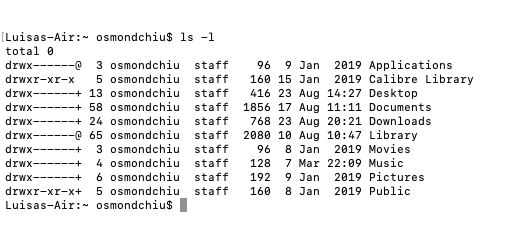
\includegraphics[width=10cm]{Screenshot.png}
    \label{fig:ls-1}
\end{figure}
 \par
Action:\par
Command ls -h\par
Error: None\par
Result: \par
\begin{figure}[htp]
    \centering
    
\includegraphics[width=10cm]{Screenshot2.png}
    \label{fig:ls-2}
\end{figure}
 \par
Objective: Listing recursively and by time\par
Action:\par Enter ls -R -t \par
Error: None\par
Result: The files and directories are sorted by the time of the last change\par
Objective: Absolute versus relative paths\par
Action: Test the following commands to determine what will return to the home directory of /Users/amanda/ from /Users/amanda/data.\par
\begin{itemize}
\item cd .
\item cd /
\item cd /home/amanda
\item cd ../..
\item cd ~
\item cd home
\item cd ~/data/..
\item cd
\item cd ..
\end{itemize}
\par
Error: cd . goes to the current directory, cd / goes to the root directory, cd /home/amanda goes to another directory, cd ../.. goes to /Users, cd home would go into folder name home\par
Result: cd ~, cd ~/data/..,cd, cd .. are commands that will return to the home directory of /Users/amanda/\par
Objective: Relative Path Resolution\par
Action: If pwd displays /Users/thing, enter command line ls -F ../backup\par
Error: None\par
Result: Option 4 of \begin{verbatim} original/pnas_final/ pnas_sub/\end{verbatim} because 
\begin{itemize}
\item .. moves up one file directory to users
\item /backup would move to /users/backup
\item - F would be a listing of files and folders
\end{itemize}
Objective: ls reading comprehension\par
Action: If pwd displays /Users/backup, enter command lines ls -r -F /Users/backup or ls -r -F 
Error: None\par
Result: \begin{verbatim} pnas_sub/ pnas_final/ original/\end{verbatim}\par

Objective: Creating files\par
Action:\par
Enter command \begin{verbatim}touch my_file.txt\end{verbatim}\par
Enter command ls -l\par
Error: None\par
Result: \par
\begin{figure}[htp]
    \centering
    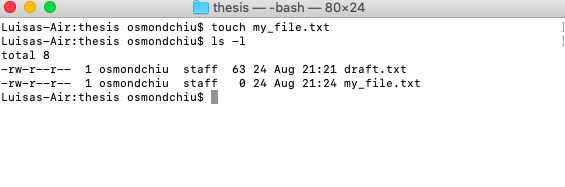
\includegraphics[width=10cm]{Screenshot3.png}
    \label{fig:ls-3}
\end{figure}

A file with nothing was created. It would be useful when there are programs that only enter output into existing files.

\subsection{Working with Files and Directories}
\subsubsection*{24/8/2019 - 11:47am}

If sucrose.dat and maltose.dat are in analysed/ but you want to move it into the current folder one up from analysed/ what is the command

\begin{verbatim}$ mv ___/sucrose.dat  ___/maltose.dat ___\end{verbatim}

Objective: Moving to the current folder\par
Action:\par
Command \begin{verbatim}$ mv ../sucrose.dat  ../maltose.dat ___\end{verbatim} \par
Error: None\par
Result: .. is the folder up so it would be moved from analysed to the folder up from it.\par


Objective: Rename statstics.txt\par
Action:\par
Command mv statstics.txt statistics.txt\par
Error: None \par
Result: File renamed statistics.txt in current folder. Other options move or copy files rather than rename it.\par

Objective: Moving and copying\par
Action:\par
Command \begin{verbatim}$ pwd
/Users/jamie/data
$ ls
proteins.dat
$ mkdir recombine
$ mv proteins.dat recombine/
$ cp recombine/proteins.dat ../proteins-saved.dat
$ ls\par\end{verbatim}
Error: None \par
Result: Only the folder recombine will be slown as proteins-saved.dat was saved in Users/jamie .\par

Objective: Using rm safely\par
Action:\par
Command\begin{verbatim}rm -i thesis_backup/quotations.txt\end{verbatim}\par
Error: None/par
Result:

\begin{figure}[htp]
    \centering
    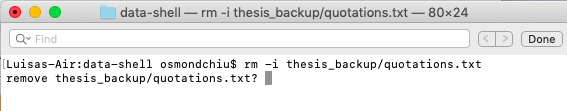
\includegraphics[width=10cm]{Screenshot4.png}
    \label{fig:ls-4}
\end{figure}

Objective: Using rm safely\label{sec: rm}\par 
Action:\par
Command\begin{verbatim}rm -i rm thesis\end{verbatim}\par
Error: Cannot remove 
Result:

\begin{figure}[htp]
    \centering
    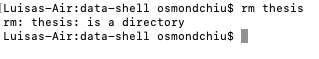
\includegraphics[width=10cm]{Screenshot5.png}
    \label{fig:ls-5}
\end{figure}

Folders cannot be removed by rm but can be with rm -r\par

Objective: Copy with multiple file names\par
Action:\par
\begin{figure}[htp]
    \centering
    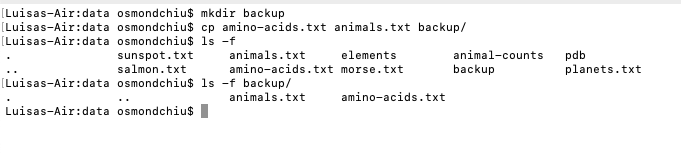
\includegraphics[width=10cm]{Screenshot6.png}
    \label{fig:ls-6}
\end{figure}
Error: None
Result: Files copied into folder\par

Objective: Copy with three file names\par\label{sec: multiplefilenames}
Action:\par
\begin{figure}[htp]
    \centering
    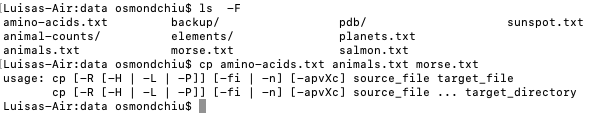
\includegraphics[width=10cm]{Screenshot7.png}
    \label{fig:ls-7}
\end{figure}

Error: Result not matching solution.\par
Result: cp: target ‘morse.txt’ is not a directory did not appear.\par

Objective: List filenames using a pattern\par
Action:\par
\begin{figure}[htp]
    \centering
    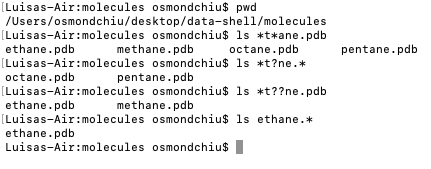
\includegraphics[width=10cm]{Screenshot8.png}
    \label{fig:ls-8}
\end{figure}
Error: None\par
Result: ls *t?ne.* produces output that matches ethane.pdb methane.pdb\par

Objective:\par Fill in blanks for wildcard exercise \par
Action:\par Enter commands\par
\begin{verbatim}$ cp *dataset* backup/datasets
$ cp 2015-11-* send_to_bob/all_november_files/
$ cp 2015-*-23-dataset* send_to_bob/all_datasets_created_on_a_23rd/\end{verbatim}
Error: None\par
Result: Files copied across.\par

Objective:\par Organising Files and Directories Exercise.\par
Action:\par
Command mv *.dat analyzed/\par
Error: None
Result: Files fructose.dat sucrose.dat moved to analysed/\par
Objective:\par Reproduce a folder structure.\par
Action:\par

Option 1:
\begin{verbatim}$ mkdir 2016-05-20
$ mkdir 2016-05-20/data
$ mkdir 2016-05-20/data/processed
$ mkdir 2016-05-20/data/raw\end{verbatim}

Option 2
\begin{verbatim}$ mkdir 2016-05-20
$ cd 2016-05-20
$ mkdir data
$ cd data
$ mkdir raw processed\end{verbatim}

Option 3
\begin{verbatim}$ mkdir 2016-05-20/data/raw
$ mkdir 2016-05-20/data/processed\end{verbatim}

Option 4
\begin{verbatim}$ mkdir 2016-05-20
$ cd 2016-05-20
$ mkdir data
$ mkdir raw processed\end{verbatim}

Error: Option 3 cannot create the two folders.\label{sec: ReproduceFolder}\par

Result: Option 1 and 2 produce the results, Option 3 is an error, Option 4 produces raw and processed in 2016-05-20, not in data.\par

\subsection{Pipes and Filters}
\subsubsection*{30/8/2019 - 8:20pm}

Objective: Distinguish between sort and sort n 

Action: Command sort n on a file with the following lines:
\begin{itemize}
\item 10 
\item 2
\item 19
\item 22
\item 6
\end{itemize}
Error: None

Result:\par
\begin{itemize}
\item 2
\item 6
\item 10
\item 19
\item 22
\end{itemize}
Only using sort will mean that it does not get sorted numerically and instead it will by based on the first digit i.e.:\par
\begin{itemize}
\item 10
\item 19
\item 2
\item 22
\item 6
\end{itemize}
Objective: Identify what the double use of greater than symbols does\par

Action:\par
\begin{figure}[htp]
    \centering
    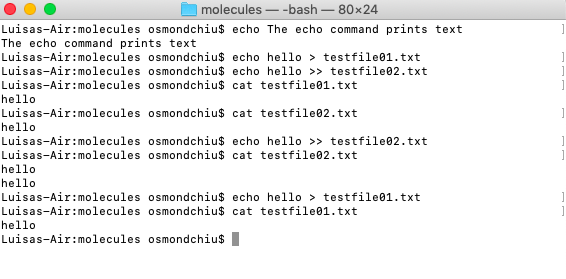
\includegraphics[width=10cm]{Screenshot9.png}
    \label{fig:ls-9}
\end{figure}
Error: None \par
Result: Compared to a single greater than symbol, a double use will not overwrite but add additional lines into documents

Objective: Appending data

Action:

Command \begin{verbatim}head -n 3 animals.txt > animals-subset.txt\end{verbatim}

Command \begin{verbatim}tail -n 2 animals.txt >> animals-subset.txt\end{verbatim}

Error: None

Result: animals-subset.txt will be the first three lines and last two lines from animals.txt or Option 3.\par

Objective: Piping Commands Together\par

Action:\par
\begin{figure}[htp]
    \centering
    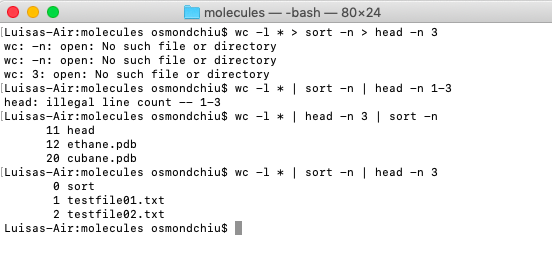
\includegraphics[width=10cm]{Screenshot10.png}
    \label{fig:ls-10}
\end{figure}
Error: None \par

Result: Option 4 has the least number of lines

Objective: \begin{verbatim}
 
Determine what cat animals.txt | head -n 5 | tail -n 3 | sort -r > final.txt results in\end{verbatim}\par
Action:\par
\begin{figure}[htp]
    \centering
    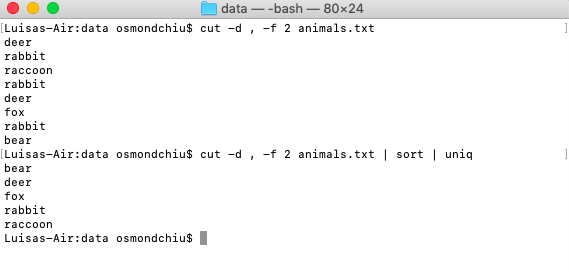
\includegraphics[width=10cm]{Screenshot11.png}
    \label{fig:ls-11}
\end{figure}
Error: None \par

Result: The first five lines of the file then the bottom three lines of those five lines then it is sorted in reverse order with that output sent to the file.\par

Objective: Construct pipeline to filter out adjacent matching lines in a file

Action:\par
\begin{figure}[htp]
    \centering
    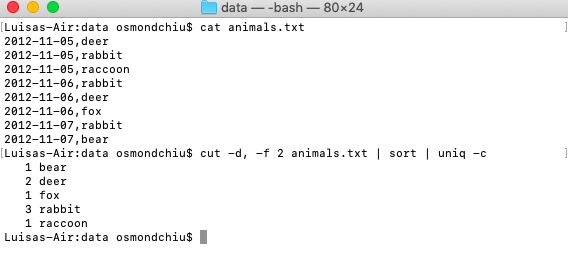
\includegraphics[width=10cm]{Screenshot12.png}
    \label{fig:ls-12}
\end{figure}

Result: Duplicates of rabbit removed

Objective: Determine which pipe to count number of times

Action:\par
\begin{figure}[htp]
    \centering
    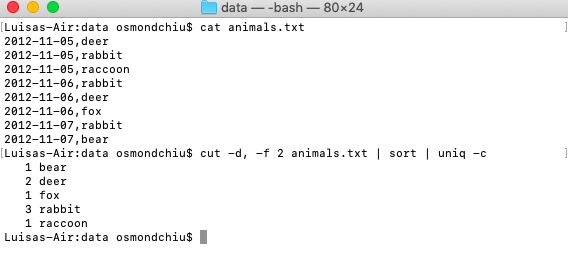
\includegraphics[width=10cm]{Screenshot13.png}
    \label{fig:ls-13}
\end{figure}

Error: None

Result: Option 4 is the correct one because cut -d breaks up the two columns, -f 2 animals.txt then chooses the 2nd column. It then needs sort for the adjacent line count command of uniq -c

Objective: Wildcat expressions as alternative to  *[AB].txt

Action:

Commands ls *A.txt and ls *B.txt  

Result: The output from tls *A.txt and ls *B.txt are separated because there are two commands.

If there were no *A.txt or *B.txt files, it would generate an error.

Objective: Removing unneeded files if raw files end in .dat and the processed files end in .txt

Action: Command rm *.txt

Error: None

Result: All the processed files ending in .txt would be removed and all the raw files of .dat would remain

rm ?.txt would only remove .txt with one character names, rm * .txt would delete all files and a .txt named file, rm *.* would delete all files.


\subsection{Loops}
\subsubsection*{30/8/2019 - 9:44pm}

Objective: Variables in Loops

Action:\par
\begin{figure}[htp]
    \centering
    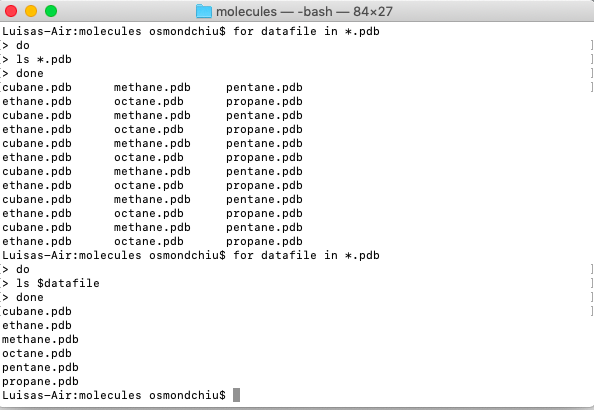
\includegraphics[width=10cm]{Screenshot14.png}
    \label{fig:ls-14}
\end{figure}

Error: None

Result: The first code lists all files ending in .pdb and loops the action it whereas the second code loops the listing of a file

Objective: Limiting Set of Files 

Action:\par
\begin{figure}[htp]
    \centering
    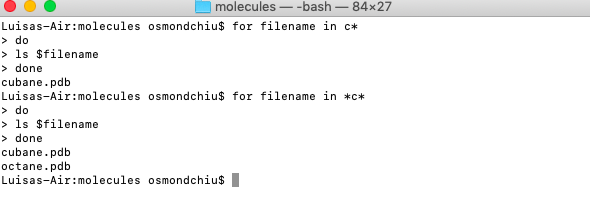
\includegraphics[width=10cm]{Screenshot15.png}
    \label{fig:ls-15}
\end{figure}

Error: None

Result: Only cubane.pdb is listed after first code run and only cubane.pdb and octane.pdb will be listed after second code run.


Objective: Answer Saving a File to a Loop - Part 1 Exercise\par
Action:\par
\begin{figure}[htp]
    \centering
    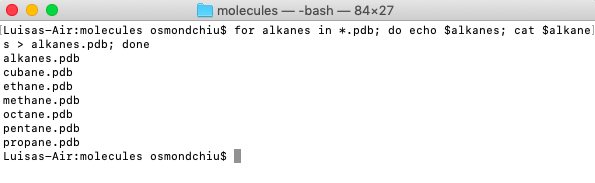
\includegraphics[width=10cm]{Screenshot16.png}
    \label{fig:ls-16}
\end{figure}

Error: None

Result: Files  cubane.pdb, ethane.pdb, methane.pdb, octane.pdb, pentane.pdb and propane.pdb are printed. The loop and single greater than means overriding until the text from propane.pdb is the final text saved to a file called alkanes.pdb.

Objective: Answer Saving a File to a Loop - Part 1 Exercise\par
Action:\par
\begin{figure}[htp]
    \centering
    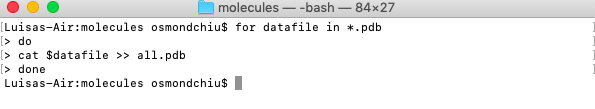
\includegraphics[width=10cm]{Screenshot17.png}
    \label{fig:ls-17}
\end{figure}

Error: None

Result: Files cubane.pdb, ethane.pdb, methane.pdb, octane.pdb, pentane.pdb and propane.pdb are concatenated and saved to a file called all.pdb with no overriding of text.

Objective: Identifying Difference (Dry Run Exercise)\par
Action: Examine the two scripts\par
\begin{figure}[htp]
    \centering
    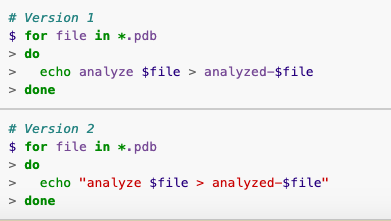
\includegraphics[width=10cm]{Screenshot18.png}
    \label{fig:ls-18}
\end{figure}

Result: The first script will run code, directing output whereas the second script will print everything within the quotation marks. The second script will do the dry run.

Objective: Nested Loops\par
Action: \par
\begin{figure}[htp]
    \centering
    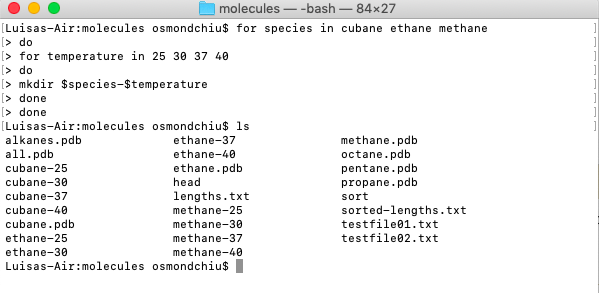
\includegraphics[width=10cm]{Screenshot19.png}
    \label{fig:ls-19}
\end{figure}

Result: For each value listed in species loop, the other look through the list of temperatures, and has created a new directory for each combination.

\subsection{Shell Scripts}
\subsubsection*{31/8/2019 - 4:27pm}

Objective: List unique species

Action:

Command nano species.sh\par 
Enter in the following commands

\begin{verbatim}
for file in $@
do
	echo "Unique species in $file:"
	cut -d , -f 2 $file | sort | uniq
done \end{verbatim}
Save species.sh

In data-shell/data/animal-counts/ run command bash species.sh *.*

Result:

\begin{figure}[htp]
    \centering
    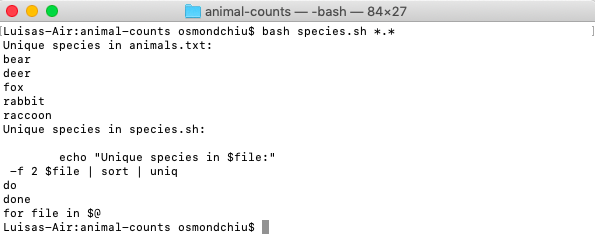
\includegraphics[width=10cm]{Screenshot20.png}
    \label{fig:ls-20}
\end{figure}

Objective: Explain Why Record Commands in the History Before Running Them?

Explanation: A command of history | tail -n 5 > recent.sh would save the last five lines of script. This would be handy in case the command causes a problem such as a crash. Recording it after may lose it.

Objective: Variable in shell scripts

\begin{figure}[htp]
    \centering
    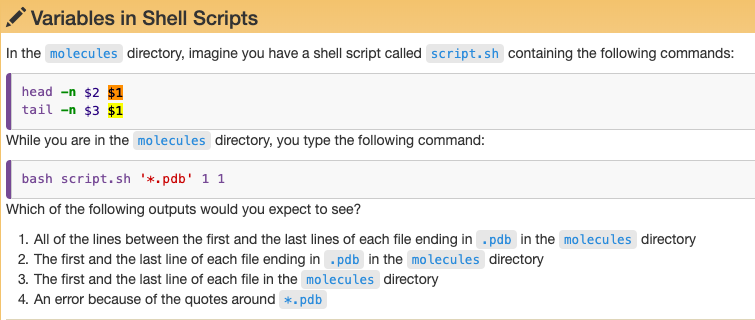
\includegraphics[width=10cm]{Screenshot21.png}
    \label{fig:ls-21}
\end{figure}

Explanation: The correct answer is Option 2 as \$2 is 1 and \$1 is '*.pdb' and \$3 is 1 and \$1 is '*.pdb'. 

The command would then be head -n 1 cubane.pdb ethane.pdb octane.pdb pentane.pdb propane.pdb
and tail -n 1 cubane.pdb ethane.pdb octane.pdb pentane.pdb propane.pdb

Objective: Find the Longest File With a Given Extension

Explanation: The following command in longest.sh would  print the name of the .pdb file in /tmp/data that has the most lines if bash longest.sh /tmp/data pdb was used.

\begin{verbatim}wc -l $1/*.$2 | sort -n | tail -n 2 | head -n 1\end{verbatim}

Word count organised by number of lines in /tmp/data/*.pdb sorted numerically then filtered by last two lines of output then the top one.

Objective: Script reading comprehension

\begin{figure}[htp]
    \centering
    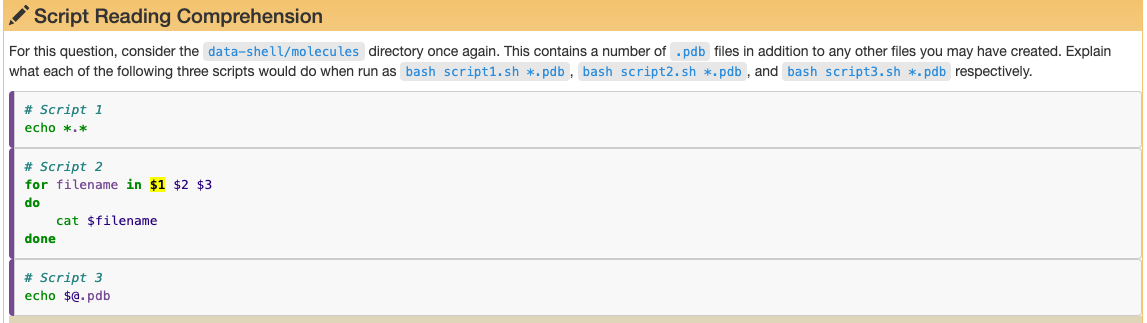
\includegraphics[width=10cm]{Screenshot22.png}
    \label{fig:ls-22}
\end{figure}

Explanation: Script 1 prints out a list of all files containing a dot in their name. 

Script 2 prints the contents of the first 3 .pdb files. 

Script 3 prints out all the script, followed by .pdb

Objective: Debugging script

\begin{figure}[htp]
    \centering
    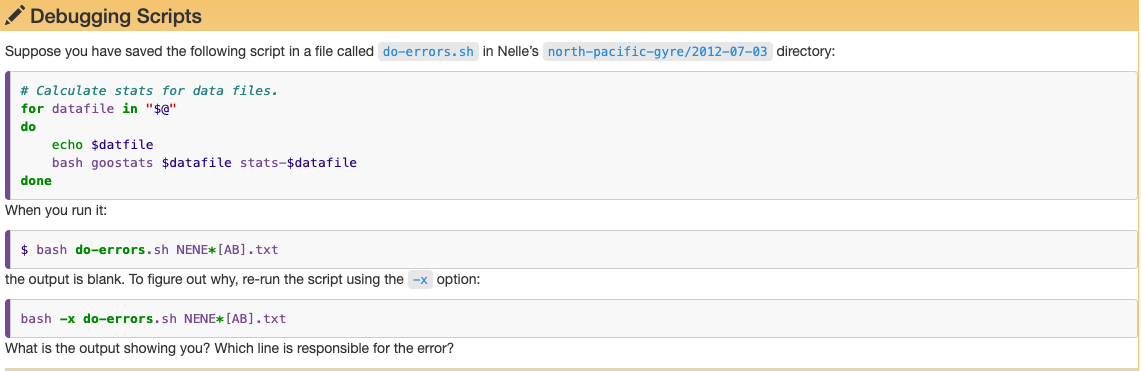
\includegraphics[width=10cm]{Screenshot23.png}
    \label{fig:ls-23}
\end{figure}

Explanation: The error is datfile because it is a typo so echo would not make it print anything

\subsection{Finding Things}
\subsubsection*{31/8/2019 - 6:51pm}

Objective: Using Grep

Action: grep -w "of" haiku.txt

Result: "and the presence of absence"

Explanation: Option Three is correct because the use of -w limits it to the word "of" rather than a word that includes of

\subsubsection*{31/8/2019 - 9:13pm}\label{sec: Colon}

Objective: Put these commands and pipes in the right order to track species 

Error: Unclear what the purpose of the colon is or what it's impact is

Objective: Count how many times the sisters are mentioned in LittleWomen.txt 

Action: 

cd data-shell/writing/data/

\begin{verbatim}
    for sis in Jo Meg Beth Amy
do
	echo $sis:
	grep -ow $sis LittleWomen.txt | wc -l
done
\end{verbatim}

Result:

\begin{figure}[htp]
    \centering
    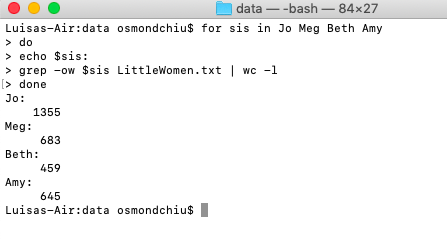
\includegraphics[width=10cm]{Screenshot24.png}
    \label{fig:ls-24}
\end{figure}

Jo was mentioned the most times.

Objective: Matching and subtracting to find all files in /data whose names end in s.txt (e.g., animals.txt or planets.txt), but do not contain the word net

Action:

\begin{figure}[htp]
    \centering
    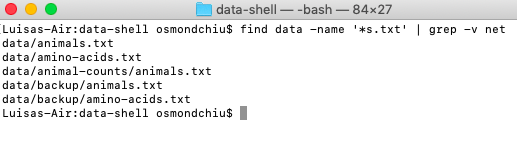
\includegraphics[width=10cm]{Screenshot25.png}
    \label{fig:ls-25}
\end{figure}

Result: Option 1 is the only correct option.

Option 2 expands the shell so find doesn't work properly.

Option 3 searches for file contents for not having 'temp'


Objective: Explain the following pipeline command

\begin{verbatim}
wc -l $(find . -name '*.dat') | sort -n    
\end{verbatim}

Explanation: Line count for all .dat files in directory and subdirectories sorted numerically


Objective: Finding Files With Different Properties

Explanation: The command would be find ./ -type f -mtime -1 -user ahmed.

Find . would search any name with -type f specifying file and mtime -1 in the last day with -user being ahmed.


\newpage

\section{Proof of Concept - Scoping}
\subsubsection*{10/8/2019 – 10:57am}
I’ve started to have a think about the proof of concept for scoping.\par
There are a range of jobs that will need to be done for my thesis, including a fair few tedious and repetitive tasks. Automating some of those processes would free up time and help a lot.\par
Given my thesis is about re-nationalisations in Australia, it will involve a fair bit of trawling for information through Trove, government documents, websites and newspapers. From what I can tell to date, there is not much on re-nationalisation in Australia but plenty on problems with privatisation. Identifying examples of re-nationalisations to examine and available sources would be very useful.\par
There is also the more general tasks of formatting and referencing and task management.
\subsection{Jobs, Pains and Gains }
\subsubsection*{12/8/2019 - 9:55pm}
Reflecting on my scoping project, there are plenty of obvious tasks and pain points for the thesis though the technical solutions are less immediately obvious.\par
Going through the range of tasks that need to be done for my thesis, there are quite a few. These include developing my research question to data collection to data analysis to writing and editing and referencing. It will be time consuming and I will also need to balance it with other work and personal commitments.\par
There are some obvious tools that can be used to ease pain that were mentioned during the class such as LaTex, Github, referencing and project management software.\par
Opportunities for gain would be through automating searches. The limited academic literature on re-nationalisation in Australia means that it would be handy if it could trawl through Trove and other newspaper archives, especially over the last decade. It may be a better source for information than academic journals.
\subsection{Creating a Document in LaTex}
\subsubsection*{14/8/2019 - 7:30pm}
I’ve decided to try to use LaTex for my scoping project. I had initially drafted my scoping project on Word but will copy the text over.\par
I have not used LaTex before but playing around with it, the commands for basic formatting does not look too difficult to remember. I quickly looked at the guides on Overleaf.\par
I created a new blank document then started from scratch by removing the existing code.\par
Objective: Generate Title and author\par
Action:

\begin{verbatim}\title{Proof of Concept Scoping Exercise}|
\author{Osmond Chiu}
\maketitle
\end{verbatim}
\par
Click ‘compile’\par
Error: Compile error\par
Result: No document generated\par
I remembered that I needed to include the type of document and also to say beginning and end.\par
Objective: Generate document with title and author\par
Action:
\begin{verbatim}\documentclass{article}
\title{Proof of Concept Scoping Exercise}
\author{Osmond Chiu}
\begin{document}
\maketitle
\end{document}
\end{verbatim}
Error: None\par
Result: Generated document with title, author and current date\par
I was surprised that the date appeared as I did not include the command for date. I assume this is automatic for the date it was compiled.\par
The next step was organising my contents by creating headings, subheadings and bullet point lists.\par
Objective: Create section and section headings\par
Action:
\begin{verbatim}
\subsubsection*{Planned Thesis Topic}
\subsubsection*{Tasks to be done for thesis}
\subsubsection*{Potential pain points}
\subsubsection*{Data Collection}
\subsubsection*{Data Analysis}
\subsubsection*{Writing}
\subsubsection*{Work Commitments}
\subsubsection*{Potential pain relievers}
\subsubsection*{Managing Tasks and Work Commitments}
\subsubsection*{Writing}
\subsubsection*{Referencing and formatting}
\subsubsection*{Out of scope}
\subsubsection*{Opportunities to make gains}
\subsubsection*{Data Collection}
\end{verbatim}
Error: None\par
Result: Section and section headings created without numbers\par
Objective: Create itemised lists\par
Action:\par
There are a range of tasks that will need to be done for my thesis. The tasks will include (but not be limited to):
\begin{itemize}
\item Developing a research question and plan;
\item Writing my research proposal;
\item Collecting data;
\item Doing a literature review;
\item Analysing the data;
\item Writing a dissertation plan
\item Writing my first draft;
\item Editing the draft;
\item Proofing; and
\item Referencing and doing a bibliography.
\end{itemize}
Collecting data and doing the literature review will involve (but not be limited to):
\begin{itemize}
\item Compiling a list of examples of re-nationalisation in Australia and finding relevant further background information;
\item Identifying key Australian case studies to explore in further detail including the broader socio-economic context;
\item Collating existing literature on re-nationalisations in Australian and overseas; and
\item Developing questions and conducting interviews with key individuals and organisations involved in Australian case studies.
\end{itemize}
Analysing data may involve (but not be limited to):
\begin{itemize}
\item Coding data on key factors applicable to re-nationalisations to identify any patterns;
\item Applying theoretical frameworks to determine if they provide good explanations for re-nationalisations; and
\item Examining interview transcripts to identify any common themes mentioned by interviewees.
\end{itemize}
Error: None\par
Result: Itemised lists generated\par
The thing that is unclear is how to easy leave a space between lines without needing to specify how large the gap is.
\subsection{Uploading Scoping Project}
\subsubsection*{14/8/2019 - 10:30pm}
After editing the text of my scoping project, it is now ready to be submitted. I will need to download it as a PDF and also in tex format.\par
Objective:\par Download LaTex document as PDF\par
Action:\par
Click ‘recompile’\par
Click Download PDF\par
Error: None\par
Result: Downloaded PDF\par
The downloaded PDF was then submitted via iLearn\par
Objective:\par
Download tex file\par
Action:\par
Click ‘Menu’\par
Under Download, click ‘Source’\par
Error: None\par
Result: No download.\par
It wasn’t clear what happened. I tried it a few times but it did not appear on my system even though it appeared to download. I changed browsers from Safari to Chrome and it seemed to work. Unclear why.\par
The downloaded .tex file was then uploaded to Cloudstor
\subsection{Revising Scoping Exercise}
\subsubsection*{16/08/2019 - 7:01pm}
After re-examining the guidance Week 2 in Cloudstor, I did some additional editing of my scoping exercise to remove references to tools and to focus on the jobs, pains, pain relievers, gains and gain opportunities.\par
The revised version was uploaded by repeating the previous steps I had taken.
\subsection{Pasting Text into LaTex}
\subsubsection*{19/8/2019 - 6:04pm}
I've decided to shift my Learning Journal over from Word to Overleaf. I copied and pasted the text from Word into a blank document. During the editing process I have a few errors, some of which I could resolve, others which I have not resolved yet:\par
\textit{Underscores and bullet points do not work}\label{sec: Underscore}\par
An attempted list does not work and all the bullet points are in a single line. I tried to work out why this error was occurring and realised it was because of the inclusion of underscores. I resolved the issue by replacing the underscores with a space.\par
\textit{Commands}\label{sec: Commands}\par
It was initially unclear how to include commands in LaTex without executing them when I copied across the text for the learning journal. I entered 'how to display latex commands in latex' into Google and an Overleaf FAQ page that suggested using  \begin{verbatim}\begin{verbatim} \end{verbatim} \par
\textit{Paragraphs}\label{sec: Paragraphs}\par
I had initially used  \begin{verbatim}\par\end{verbatim} to create paragraphs but it was not able to create a space between lines. Looking through the FAQ, I found that using the double backslash could do it.\par
Noticing the warnings in the log and output file, after guidance from the lecture, I looked at \begin{verbatim}https://www.overleaf.com/learn/latex/Paragraph_formatting\end{verbatim} and determined I could replace the double backslash with a \begin{verbatim}\par\end{verbatim} and insert the following code \begin{verbatim}\setlength{\parindent}{0em}
\setlength{\parskip}{1em}\end{verbatim}

\textit{Italics}\par
To distinguish the commands to execute, I attempted to italicise slabs. Because of the use of brackets in multiple commands it became very difficult to close the formatting. I gave up for the time being but will reinvestigate.\par
\textit{Table of Contents}\par
I have attempted to create a table of contents using 'Chapters' but it does not seem to be working. As a work around, I have used 'Sections' instead.

\section{Proof of Concept - Elaboration}

\subsection{Computational thinking}
\subsubsection*{19/8/2019 - 6:04pm}
Applying 'computation thinking' to my scoping exercise to break down pains and gains into smaller parts.\par 
The pains are:
\begin{itemize}
\item Research plan
\item Data collection
\item Literature review
\item Coding data
\item Analysing data
\item Writing
\item Editing and proofing
\item Formatting
\item Referencing 
\end{itemize}
The opportunities for gain are:
\begin{itemize}
\item Research plan
\item Data collection
\item Literature review
\item Formatting
\item Referencing
\end{itemize}
What are the patterns in the problems and how can the solutions be revised to produce a step-by-step guide?
\subsection{Out of Scope}
\subsubsection*{21/8/2019 - 9:04pm}
The feedback from my initial scoping exercise was that it did not include what was outside the scope of the project.\par
I identified a few jobs that I stated were pains that were ultimately jobs requiring human judgement. They were 
\begin{itemize}
\item making decisions that influence data collection such as the scope of my research question or definitions of re-nationalisation
\item analysing summarised sources for literature reviews
\item trying to apply broader theoretical frameworks
\item understanding the broader context to case studies
\item involving others in proofing and editing
\end{itemize}
\subsection{Decomposing Gains}
\subsubsection*{21/8/2019 - 9:32pm}
I have examined the Gains I included in my scoping exercise to break them down into smaller more manageable tasks. It appears there will be some overlap with Pains.

\subsection{Computational Analysis for Data Collection}
\subsubsection*{22/8/2019 - 8:01pm}
I have decided that the automation of data collection will be the achievable process for my Proof of Concept.\par
This was on the basis of excluding jobs that involved human judgement and that there may be some more obvious off-the-shelf solutions for other pain relievers and gains. Automating it will have the maximum gain in terms of improved research as well as saving time.\par
I have broken the job down into the following tasks that need to be stepped out:
\begin{itemize}
\item Defining the research aim
\item Determining keywords for research
\item Identifying available sources
\item Researching what tools interact with those sources
\item Testing the tools
\item Using the tools for research
\item Saving sources
\item Organising sources
\item Analysing sources
\item Producing metadata
\item Deciding if the process needs to be repeated because the research aim is not met
\end{itemize}
\subsection{Elaboration - Data Collection}
\subsubsection*{26/8/2019 - 9:00pm}

Based on the algorithm, the steps that technology could assist with are using the tools for research, saving sources, organising sources and producing metadata.\par

Because of the limited information in journals, I have decided to focus the elaboration on searching newspaper articles. The parameters of keywords in article text and restricting it to Australian newspapers should be sufficient.\par

I know an API exists for Trove which may make a pipeline easier but I am not sure what customised script will be needed. Also the more recent newspaper archives are in ProQuest or Factiva which it is unclear if there is an API or if there will be copyright issues. There is more information about what privatisation occurred in the past 30 years which makes it easier to navigate even if there is no API.\par

I am less clear about exporting, saving and organising the sources. I imagine script with customised command lines can do this but need further guidance.\par

\subsection{Elaboration - software}
\subsubsection*{22/8/2019 - 8:01pm}

Reflecting on my initial Proof of Concept, I might be limited in what I can do. A conversation on the Slack channel suggested a backup so I have outlined using bibliographic software to organise sources.\par
Keeping organising sources by including tags and notes would minimise re-reading and also make it easier to cite and refer.\par
I have also taken the computational thinking and elaboration section out of the Proof of Concept document and placed it into a separate one.\par

\subsection{Elaboration - Text Analysis}
\subsubsection*{2/9/2019 - 8:45pm}

After some advice and research, it seems ProQuest and Factiva do not have an API and that any automated searches might require payment. As most re-nationalisations started in the latter half of the 1990s, there would not be few articles in Trove meaning it would not be useful to try using the API for it. This means that using tools for data collection for my thesis will be difficult.

Re-examining the algorithm, the other steps that might be aided by a tool are analysis or the organisation of sources.

Following advice, I tested Voyant Tools to see if text analysis. I used ProQuest to identify three articles on the Port Macquarie Base Hospital going back into public control in the mid-2000s.

Objective: Test Voyant Tools for suitability

Action: 

Go to https://voyant-tools.org/\par
Uploaded three articles on Port Macquarie Base Hospital\par
Click 'Reveal'\par

Result:

\begin{figure}[htp]
    \centering
    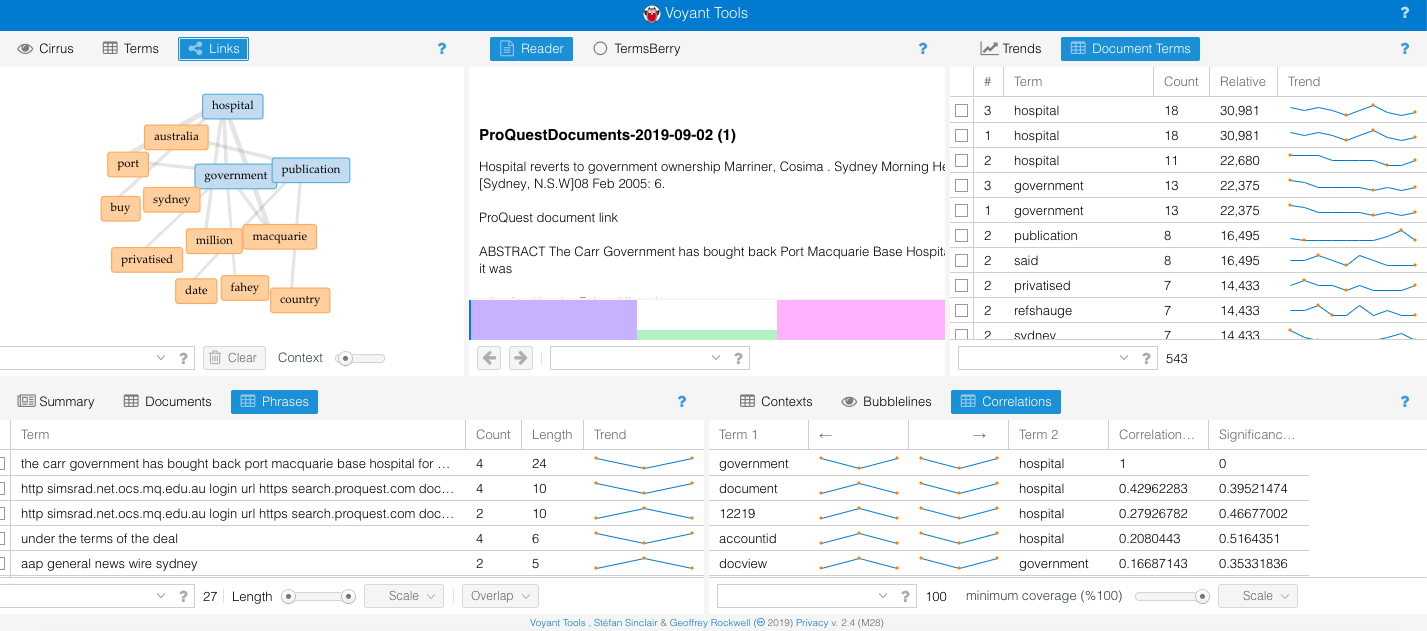
\includegraphics[width=10cm]{Screenshot26.png}
    \label{fig:ls-26}
\end{figure}

The results were of limited value as the common terms of 'privatisated', 'government', 'hospital' would not help in analysis. Other forms of visualisations or correlations did not appear to be useful.

Based on this, it seems that a text analysis tool might not be useful. Using a tool for the organisation of sources, including tagging, grouping related sources and notes, might be most useful. One tool that could aid would be NVivo, however, it is not an open source tool. 

An open source tool with both the tagging and text analysis features is Open Semantic.

It is unclear from a search of its website and via search engines of the terms bibliography, referencing and citations, as to whether it can be exported. It seems likely that a bibliography tool will still be needed.

\subsection{Elaboration - Organising Data}
\subsubsection*{3/9/2019 - 9:15pm}


Objective: Test Open Semantic Search

Action:
\begin{itemize}
\item Downloaded the installation first
\item Download Virtual Box
\item Install Virtual Box
\end{itemize}

Error: System Extension Blocked

Result: Virtual Box still appears to work

Action: 
\begin{itemize}
\item Open Virtual Box
\item Click file then Import Appliance
\item Select Open Semantic Search.ova and click import
\item Once import complete, go to settings and add folder "Thesis"
\end{itemize}

Error:\label{sec: SecurityPrivacy}

\begin{figure}[htp]
    \centering
    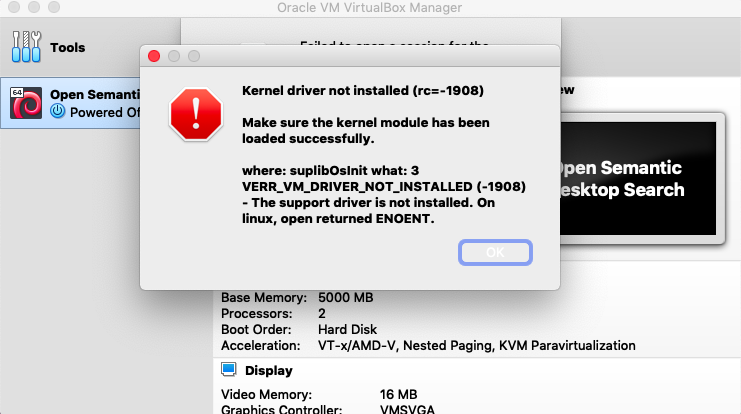
\includegraphics[width=10cm]{Screenshot27.png}
    \label{fig:ls-27}
\end{figure}

Result:

Open Semantic Search does not work and Virtual Box crashes. It will require more testing to work out how the problem is fixed.

Action:

\begin{itemize}
\item Google "kernel driver not installed (rc=-1908) mac"
\item Click on
https://medium.com/@Aenon/mac-virtualbox-kernel-driver-error-df39e7e10cd8 and read instructions
\item Go to System Preferences then Security \& Privacy then click Allow
\item Restart VirtualBox
\item Ensure the Open Semantic Search is selected as a tool then click the start icon
\end{itemize}

Error: Screen is stuck on "Waiting until Solr server is up and loaded the core" for over half an hour. 

Result: Open Semantic Search is running but it is a slow lagging program. It is unclear if it is due to my older laptop or another issue.

Objective: Test Hypothes.is

Action:
\begin{itemize}
\item Download Chrome extension
\item Set up Hypothes.is account
\item Search for PDF document on privatisations
\item Click Hypothes.is icon on browser toolbar to activate
\item Highlight lines, tag and add notes
\item Check Hypothes.is account to see if data is transferred across.
\end{itemize}

Error: None

Result:

\begin{figure}[htp]
    \centering
    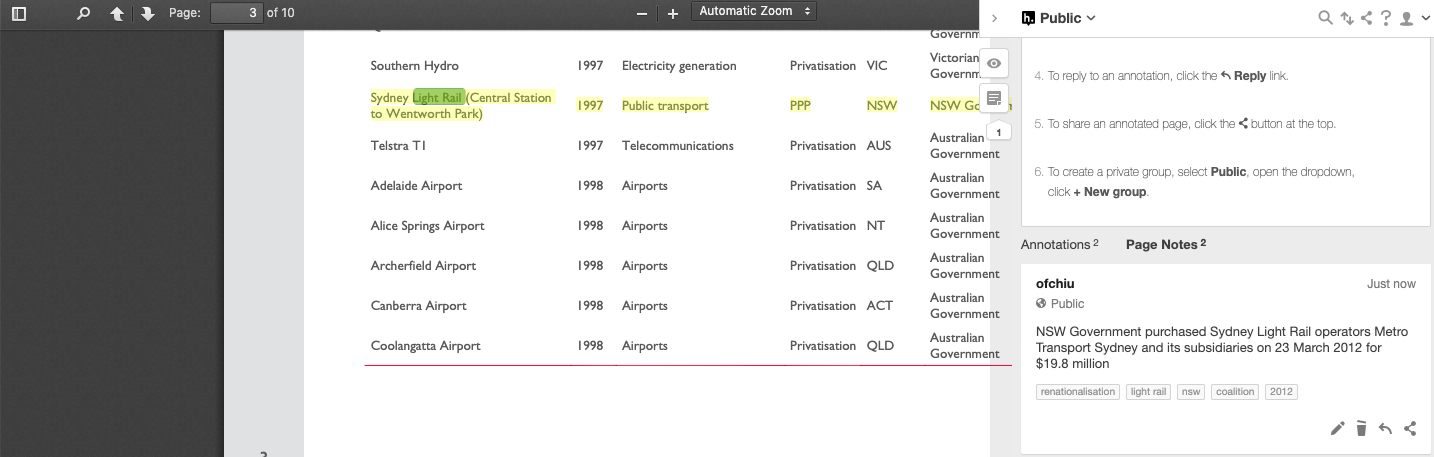
\includegraphics[width=10cm]{Screenshot28.png}
    \label{fig:ls-28}
\end{figure}


\begin{figure}[htp]
    \centering
    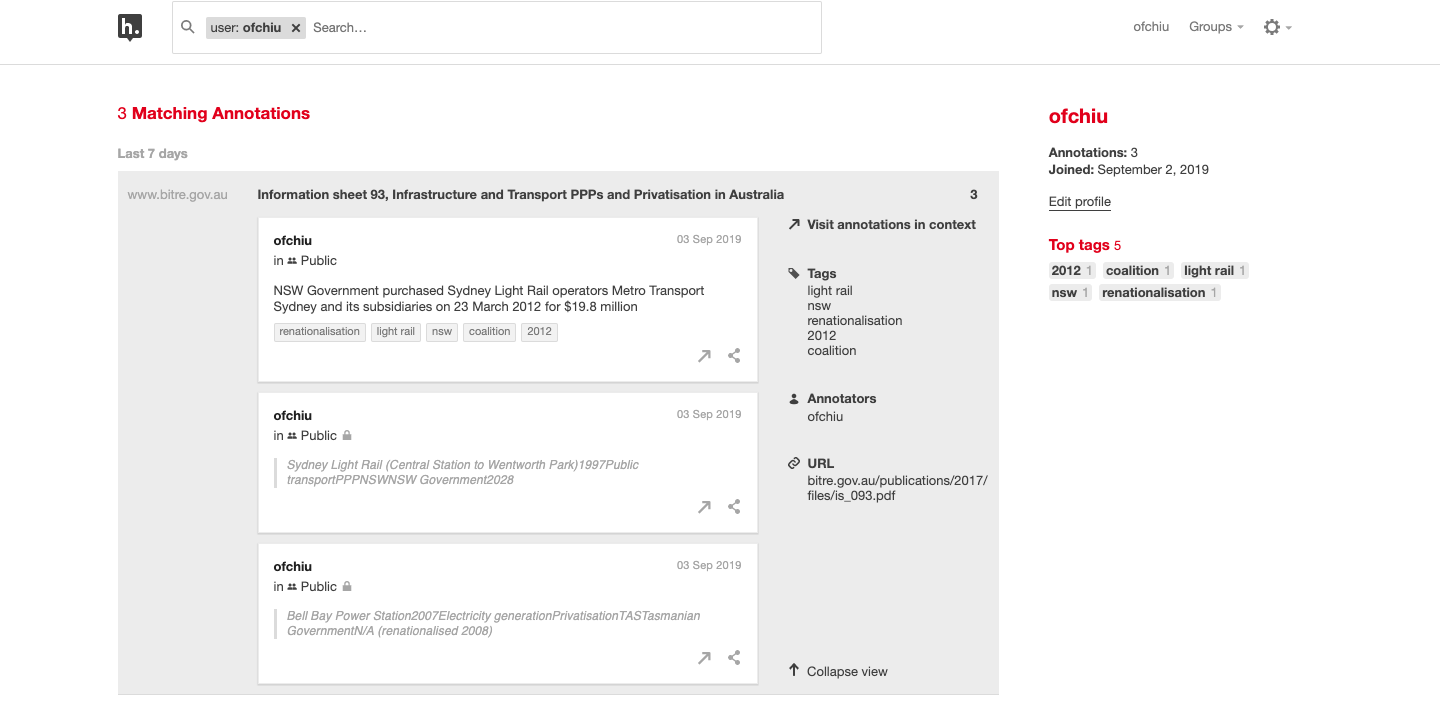
\includegraphics[width=10cm]{Screenshot29.png}
    \label{fig:ls-29}
\end{figure}

The highlighted lines and tags transferred across to Hypothes.is.

Hypothes.is is limited to the web which means I will not be able to tag PDFs I have downloaded from the web. This might be a problem for any newspaper articles downloaded from Factiva, ProQuest or journal articles.

Based on the documentation at \begin{verbatim} https://www.zotero.org/support/adding_items_to_zotero\end{verbatim} There does not appear to be an easy way to transfer saved files to Zotero or other bibliography software. It can be exported using an API at https://jonudell.info/h/facet/?max=50

Objective: Test Zotero

Action:

\begin{itemize}
\item Install Zotero and browser add-on
\item Open Zotero
\item Create new collection 'Thesis'
\item Go to Macquarie Library website and search for 
\item Download Bibtex for book
\item Click File then Import Bibtex
\item Move imported reference to collection
\item Tag and add a note to
\item Go to PDF in browser and click on toolbar icon
\item Select collection, add tags and accept
\item Repeat process with a HTML webpage
\end{itemize}

Result:

\begin{figure}[htp]
    \centering
    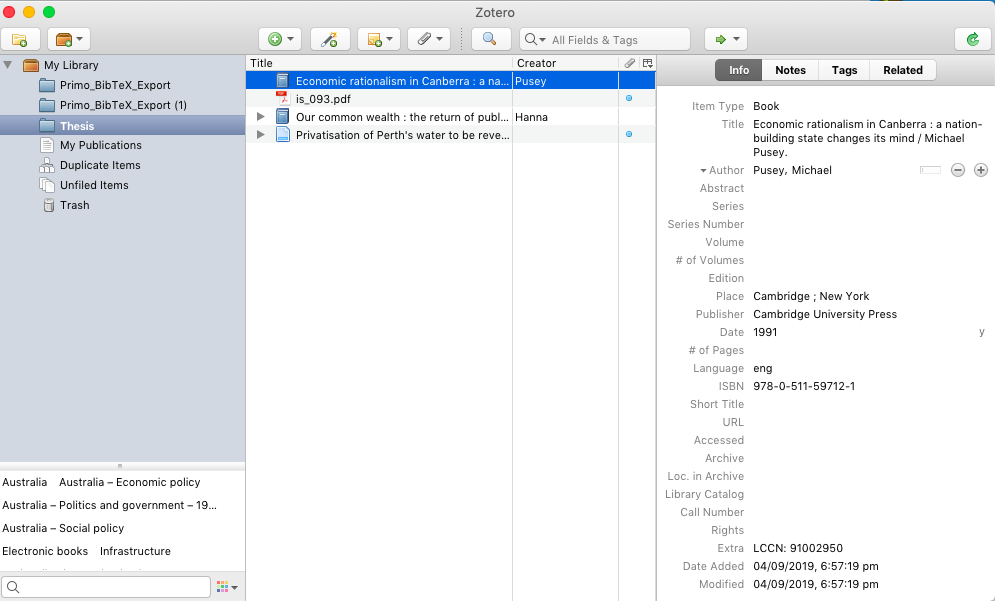
\includegraphics[width=10cm]{Screenshot30.png}
    \label{fig:ls-30}
\end{figure}

The importation of Bibtex files worked but data will need to be cleaned e.g. title.

The webpage and PDF were added to Zotero via the browser but without a lot of citation information. This will need to be manually added. 

Searches can be made via the tags and links can be made between referred sources.

\subsection{OpenSemantic}
\subsubsection*{7/9/2019 - 3:00pm}

OpenSemantic Search is now working, it was lagging because of limited memory. The issue was limiting the available memory to below 1GB.

While it works, it still is lagging. It will need to be further tested to see if it is a valuable tool or useful for the Proof of Concept.

\section{Proof of Concept - Design Document}
\subsection{Creating User Stories}
\subsubsection*{9/9/2019 - 6:40pm}

Based on the elaboration, organisation of data and referencing will be the Proof of Concept.

I have identified the following user stories:
\begin{itemize}
\item Index
\item Text Search
\item Creating Tags
\item Tagging Documents
\item Highlights
\item Annotations
\item Import annotations
\item Import references
\item Insert references
\item Generate bibliography
\end{itemize}

The programs used will be Zotero, Hypothes.is and OpenSemantic Search.

\subsection{Feedback from Elaboration Assessment}
\subsubsection*{22/9/2019 - 12:00pm}

The feedback from my Elaboration assessment was:

\textit{It is not completely clear to me how you are planning to use the tools identified. This is probably a function of the change in project focus. However, I would recommend revisiting the requirements analysis or scoping before you proceed. In order to properly assess the usefulness of Hypothes.is and Zotero you need to be clear about what you want them to actually do.
}
Reflecting on my Design Document, the aim of Hypothes.is is to tag online documents and annotate to improve the organisation of my data. The aim of Zotero will be to manage sources for referencing. 


\subsection{Disaster recovery plan}
\subsubsection*{22/9/2019 - 12:20pm}

Based on advice from the Slack channel, I have established a backup using Duplicati by connecting it to my Cloudstor account.

I have added a backup that data for Data Carpentry and the most recent Proof of Concept Design. The backup was configured to occur automatically daily.

I tested a Restore by selecting some files to be restored to a new folder called BackUp to prevent overriding and clearly distinguish the new files. The Restore occurred successfully.

A second disaster recovery option needs to be developed in case servers go down or I lose access to Cloudstor. The option can be to have it on an external hard drive or in lieu of that a USB stick that I have.

\subsection{Debugging Hypothes.is}
\subsubsection*{23/9/2019 - 7:40pm}

From Slack, a set of rules of debugging was posted:

Fail early, fail often.
Always initialize from data.
Know what it's supposed to do.
Make it fail every time.
Make it fail fast.
Change one thing at a time, for a reason.
Keep track of what we've done.
Be humble.
Test the simple things first.
And remember, a week of hard work can sometimes save you an hour of thought.

Based on it, the testing of my three tools should involve changing one obvious change at the time to force an error.

I decided to tested to see if I could annotate a non-webpage, local file using Hypothes.is that was not an online URL.

Objective: Annotating local PDF file

Action: 

Open a PDF via a web browser
Click on Hypothes.is icon on browser toolbar

Error:

\begin{figure}[htp]
    \centering
    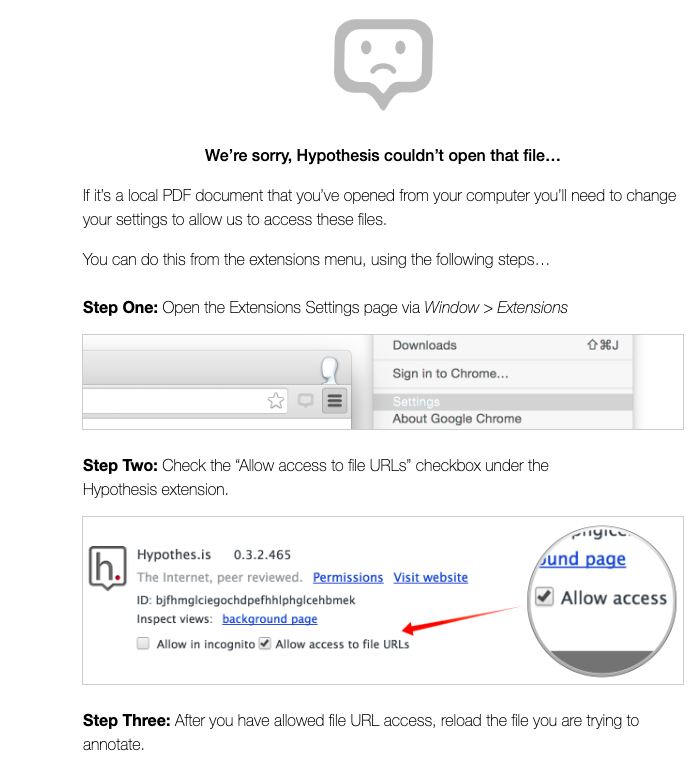
\includegraphics[width=10cm]{Hypothesistest.png}
    \label{fig:hypothesis}
\end{figure}

Result: 

I made the changes to the extension settings and re-opened the PDF in a browser. The annotation worked and it synced with Hypothes.is

I attempted to search for the location of local file via the Hypothes.is account. When I clicked, an error page was generated stating "Sorry, but it looks like this annotation was made on a document that is not publicly available." It highlighted that if a local file was annotated, I need to note its exact location and details.

\subsection{Debugging Zotero}
\subsubsection*{23/9/2019 - 9:10pm}

I decided to test what happens if I used the same tag but with capitalisation. It led to the creation of different tags.

I found a tool that allowed the renaming of tags on Hypothes.is as capitalisation will generate a different tag. I tested it, using the API token generated by Hypothes.is and it worked. The URL for the tool was https://jonudell.info/h/TagRename/

I then attempted to delete a tag from the local file. There was no easy way of deleting tags (or annotations) required re-opening the local file in a browser.

I attempted to see if it would work for Zotero in a browser. The browser toolbar did not work.

I then tested the importation of metadata into Zotero using ISBN. After successfully testing using a ISBN, I entered an incorrect ISBN to see what the effect would be. The result was a Lookup Fail error message that stated "Zotero could not find any identifiers in your input. Please verify your input and try again."

I tested the importation of a PDF to see what would occur. An error message "The selected file is not in a supported format." appeared. A similar test was done with a docx and a HTML file which had the same error message. 

\subsection{Debugging OpenSemantic Search}
\subsubsection*{24/9/2019 - 8:10pm}

I attmpted

\newpage
\section{OpenRefine}
\subsection{Working With OpenRefine}
\subsubsection*{5/9/2019 - 7:30pm}

Objective: Look for errors in 'village' column.

Action:

Scroll over to the 'village' column.
Click the down arrow and choose Facet > Text facet

Results:

Using facets, a number of errors were identified in the 'village' column:
\begin{itemize}
\item Chirdozo appears to be a mispelling of Chirodzo.
\item Ruca seems to be a mispelt Ruaca.
\item Ruaca - Nhamuenda and Ruaca-Nhamuenda. It is unclear if this is suppsoed to be Ruaca
\item The entry 49 is an error but unclear what it is.
\end{itemize}

Objective: Facets Exercise

1. Using faceting, find out how many different interview_date values there are in the survey results.

Action: Scroll over 'interview_date' column then do Facet > Text facet. 

Result: 19 different values

2. Is the column formatted as Text or Date?

Result: Text

3. Use faceting to produce a timeline display for interview_date. 

Action:

Use 'Edit cells' then 'Common transforms' then 'To date' to convert this column to dates.

Result: 

\begin{figure}[htp]
    \centering
    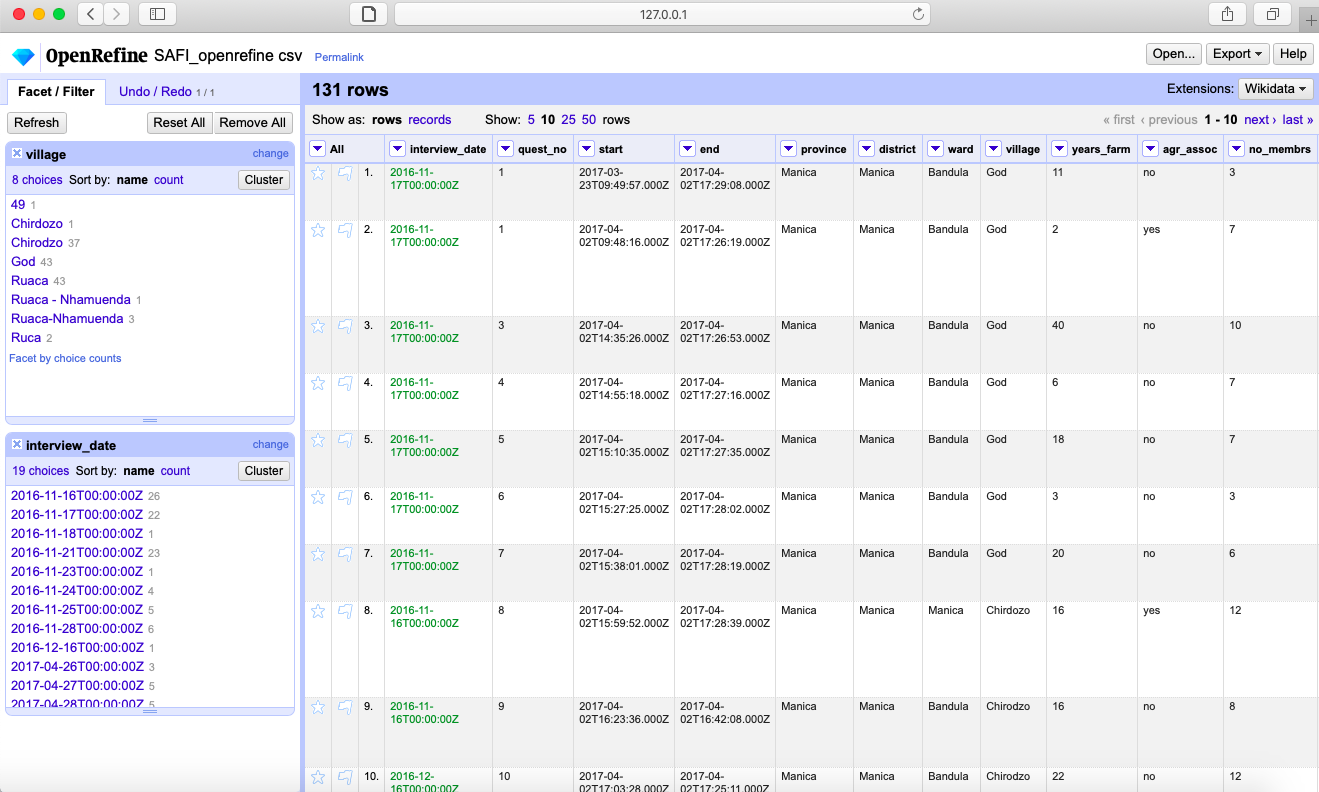
\includegraphics[width=10cm]{Screenshot31.png}
    \label{fig:ls-31}
\end{figure}


4. During what period were most of the interviews collected?

Result: 

\begin{figure}[htp]
    \centering
    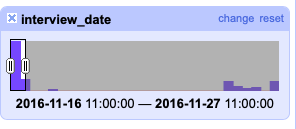
\includegraphics[width=10cm]{Screenshot32.png}
    \label{fig:ls-32}
\end{figure}

Mostly November 2016

Objective: Transform data in items owned column

Action:

Click on Column Name, Edit Cells Then Transform\par
Enter value.replace("'", "")\par
Click ok\par
Repeat process but enter value.replace("]", "")\par
Repeat process but enter value.replace(" ", "")\par

Result: Removal of brackets, single quote marks and spaces


Objective: Use Custom Text Facet

Action:

Choose Facet then Custom text facet for itemsowned column
In the Expression box, type value.split(";").
Click OK.

Result:

\begin{figure}[htp]
    \centering
    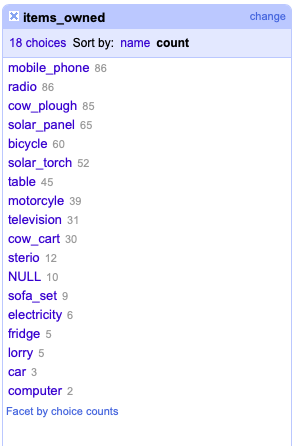
\includegraphics[width=10cm]{Screenshot33.png}
    \label{fig:ls-33}
\end{figure}


Mobile phones and radios are most common while cars and computers are least common.

Objective: Determine Which month(s) were farmers more likely to lack food?

Action: Choose Facet then Custom text and type in value.replace("[", "").replace("]", "").replace(" ", "").replace("'", "")

Result: November with 71

\subsection{Filtering and Sorting with OpenRefine}
\subsubsection*{5/9/2019 - 8:30pm}

Objective: Answer Filtering Exercise Questions

1. What roof types are selected by this procedure?

Action: After filtering, select Facet > Text facet on the respondent_roof_type column. 

Result: The roof types selected by filtering using 'mabat' are mabatipitched and mabatisloping.

2. How would you restrict this to only one of the roof types?

You need more letters in the filter to restrict to a single roof type.

Objective: Answer Sort Exercise - Sort the data by gps:Altitude. Do you think the first few entries may have incorrect altitudes?.

Action: In the gps:Altitude column, select Sort... > numbers and select smallest first.

Result: The first few entries have a value of 0 which may be used incorrectly as a missing value.

Objective: Identify what Village 49 is Exercise

Action:

Sort on gps_Longitude as a number with the largest first.
Sort on gps_Lattitude as a number with the largest first.
Using the drop down arrow on the 'village' column, select Edit column > Move column to end.
Scroll through the entries until you find village 49.
Sort only by 'interview_date' as date.
Move the 'village' column to the start of the table.

Result: Village 49 is Chirodzo as it matched the GPS coordinates and interview dates only occurred in Chirodzo on that date.

\subsubsection{Examining Numbers in OpenRefine}
\subsubsection*{6/9/2019 - 2:09pm}

Exercise Objective: Transform columns to numbers

Action: 

Click the down arrow for relevant column, then Edit cells > Common transforms… > To number.

Results: The following could be transformed to numbers

\begin{verbatim}no_members, yrs_liv, and buildings_in_compound\end{verbatim}

Village could not be transformed to numbers

\subsection{Exporting and Saving Data from OpenRefine}
\subsubsection*{6/9/2019 - 2:24pm}

Exercise Objective: Explain what the files are in an exported project and what information the files contain

Action:

Click the Export button in the top right and select Export project then go to default Download directory.

Results: Raw data plus the metadata history of changes made by project

\newpage
\section{R}
\subsection{Objects vs variables}
\subsubsection*{6/9/2019 - 3:00pm}

Exercise Question: Answer whether current content of the object areaacres is 123.5 or 6.175

Answer: areaacres is 6.175 because the areaacres calculation was not run since areahectares are redfined to 50. If it had been run after defination, it would have changed to 123.5

Exercise Question: Show that changing the values of either length and width does not affect the value of area.

Action:

length <- 1
width <- 2
area <- length * width
area
[1] 2

length <- 2
width <- 4
area

Result: [1] 2


Exercise Questions:

1. Type in ?round at the console and then look at the output in the Help panel. What other functions exist that are similar to round? 

ceiling, floor, trunc, signif

2. How do you use the digits parameter in the round function?

You place it like round(x, digits = 0)

Exercise Question: What happens when you mix different data types into a single vector?

Answer: Converted to same vector

Exercise: Mix these types in a single vector

Action:

numchar <- c(1, 2, 3, "a")
numlogical <- c(1, 2, 3, TRUE)
charlogical <- c("a", "b", "c", TRUE)
tricky <- c(1, 2, 3, "4")
class(numchar)
class(numlogical)
class(charlogical)
class(tricky)

Results:

> class (numchar)
[1] "character"
> class(numlogical)
[1] "numeric"
> class(charlogical)
[1] "character"
> class(tricky)
[1] "character"

Converted to the most common atomic vector type

Objective: Outline how many values in combinedlogical are "TRUE" (as a character) 

Action:

> numlogical <- c(1, 2, 3, TRUE)
> charlogical <- c("a", "b", "c", TRUE)
> combinedlogical <- c(numlogical, charlogical)
> numlogical
[1] 1 2 3 1
> charlogical
[1] "a"    "b"    "c"    "TRUE"
> combinedlogical
[1] "1"    "2"    "3"    "1"    "a"    "b"    "c"    "TRUE"

Result: One "True"

Objective: Complete Missing Data Exercises

1. Using this vector of rooms, create a new vector with the NAs removed.

rooms <- c(1, 2, 1, 1, NA, 3, 1, 3, 2, 1, 1, 8, 3, 1, NA, 1)
roomsno <- rooms[!is.na(rooms)]

Result is 1] 1 2 1 1 3 1 3 2 1 1 8 3 1 1

2. Use the function median() to calculate the median of the rooms vector.

The result of median(roomsno) is 1

3. Use R to figure out how many households in the set use more than 2 rooms for sleeping.

The result of roomsno[roomsno > 2] is 4

\subsection{Data Frame Exercise}
\subsubsection*{15/9/2019 - 9:27pm}

1.

\begin{verbatim} interviews_100 <- interviews[100,] \end{verbatim}

2. 
\begin{verbatim} nrow(interviews)
[1] 131
lastrow <- nrow(interviews)
interviews_last <- interviews[lastrow,]\end{verbatim}

3.

\begin{verbatim} interviews_middle <- interviews[lastrow / 2, ]\end{verbatim}

4.
\begin{verbatim} interviews_head <- interviews[-(7:lastrows), ] \end{verbatim}

\newpage

\subsection{Renaming Factors Exercise}
\subsubsection*{16/9/2019 - 7:30pm}

Objective: Rename the levels of the factor to have the first letter in uppercase: “No”,”Undetermined”, and “Yes”. 

Action:

\begin{verbatim} levels(memb_assoc) <- c("No", "Undetermined", "Yes")
plot(memb_assoc)\end{verbatim}

Result:

\begin{figure}[htp]
    \centering
    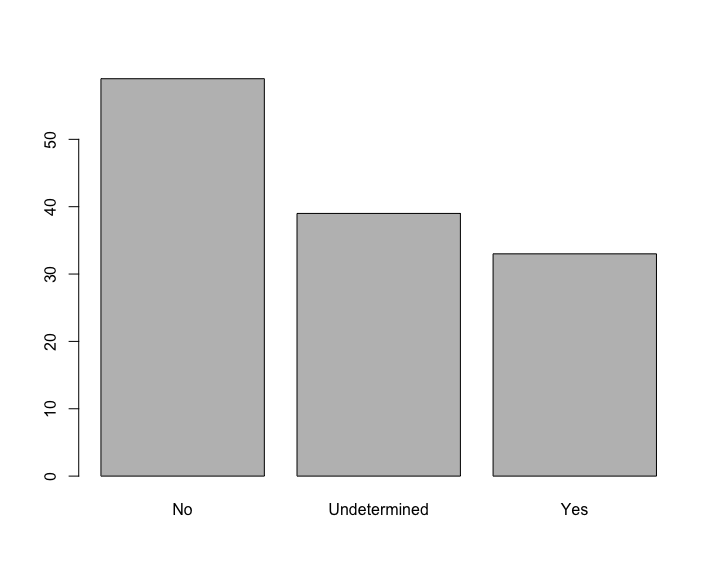
\includegraphics[width=10cm]{Screenshot34.png}
    \label{fig:ls-34}
\end{figure}


Objective: Recreate the barplot such that “Undetermined” is last (after “Yes”)

Action:

\begin{verbatim} memb_assoc <- factor(memb_assoc, levels = c("No", "Yes", "Undetermined"))
plot(memb_assoc)\end{verbatim}

Result:

\begin{figure}[htp]
    \centering
    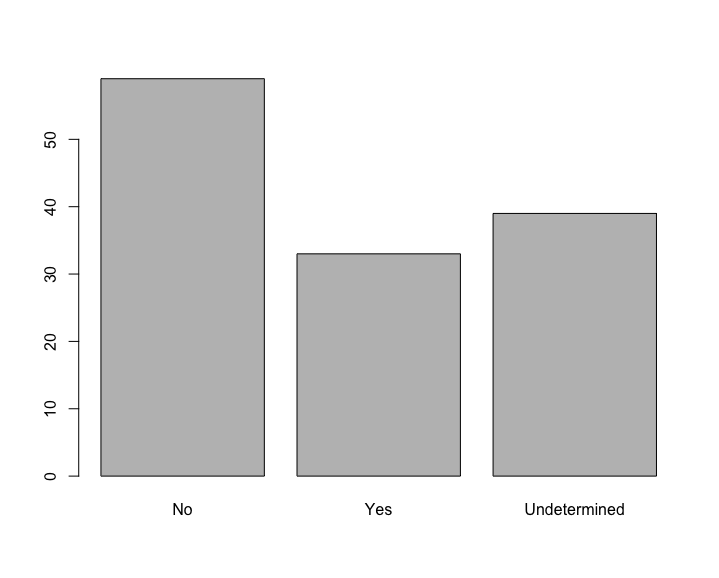
\includegraphics[width=10cm]{Screenshot35.png}
    \label{fig:ls-35}
\end{figure}

\subsection{Pipes}
\subsubsection*{16/9/2019 - 8:26pm}

N.B. think of \%$>$\% as the equivalent of 'then'

Objective: Using pipes, subset the interviews data

Action:

\begin{verbatim}
interviews %>%
filter(memb_assoc == "Yes") %>%
select(affect_conflicts, liv_count, no_meals)
\end{verbatim}
Result: Data subseted

\subsection{Mutate}
\subsubsection*{16/9/2019 - 8:35pm}

Objective: Create a new data frame from the interviews data that meet a set criteria.

Action:

\begin{verbatim}
interview_total_meals <- interviews %>% 
mutate(total_meals = no_members * no_meals) %>% 
filter(total_meals > 20) %>%
select(village,total_meals)
\end{verbatim}
Error: no_members not found. \label{sec: NoMembers}

Action:

\begin{verbatim}
interview_total_meals <- interviews %>% 
mutate(total_meals = no_membrs * no_meals) %>% 
filter(total_meals > 20) %>%
select(village, total_meals)
\end{verbatim}

Result: Data frame created

\subsection{Split-apply-combine data analysis and the summarize() function}
\subsubsection*{18/9/2019 - 8:40pm}

Objective: Find number of meals by household

Action:

\begin{verbatim}
interviews %>%
count(no_meals)
\end{verbatim}
Error: None
    
Result:

A tibble: 2 x 2
  no_meals     n
     <int> <int>
        2    52
        3    79

52 households have an average of 2 meals per day. 79 have an average of 3 meals per day. No other number

Objective: Use group_by() and summarize() to find the mean, min, and max number of household members for each village. Also add the number of observations

Action:
\begin{verbatim}
interviews %>%
group_by(village) %>%
summarize(mean_no_membrs = mean(no_membrs), min_membrs = min(no_membrs), max_membrs = max(no_membrs), ?n)
\end{verbatim}

Error: Observations do not appear\label{sec: Observations}

Result:

A tibble: 3 x 5
  village  mean_no_membrs min_membrs max_membrs ``?`(n)`                                                                 
  <fct>             <dbl>      <int>      <int> <chr>                                                                      
Chirodzo           7.08          2         12 /Library/Frameworks/R.framework/Versions/3.5/Resources/library/dplyr/help/n
God                6.86          3         15 /Library/Frameworks/R.framework/Versions/3.5/Resources/library/dplyr/help/n
Ruaca              7.57          2         19 /Library/Frameworks/R.framework/Versions/3.5/Resources/library/dplyr/help/n
 
Action:

\begin{verbatim}
    interviews %>%
    group_by(village) %>%
    summarize(mean_no_membrs = mean(no_membrs), min_membrs = min(no_membrs), max_membrs = max(no_membrs), n = n())
\end{verbatim}

Result:

  village  mean_no_membrs min_membrs max_membrs     n
  <fct>             <dbl>      <int>      <int> <int>
1 Chirodzo           7.08          2         12    39
2 God                6.86          3         15    43
3 Ruaca              7.57          2         19    49

Objective: What was the largest household interviewed in each month?

Action:

\begin{verbatim}
library(lubridate)
interviews %>%
    mutate(month = month(interview_date),
           day = day(interview_date),
           year = year(interview_date)) %>%
    group_by(year, month) %>%
    summarize(max_no_membrs = max(no_membrs))
\end{verbatim}    

Result:

A tibble: 5 x 3
 Groups:   year [2]
   year month max_no_membrs
  <dbl> <dbl>         <int>
  2016    11            19
  2016    12            12
  2017     4            17
  2017     5            15
  2017     6            15

\subsection{Reshaping with gather and spread}
\subsubsection*{18/9/2019 - 9:05pm}

Objective: Create a new data frame (named interviews_months_lack_food) that has one column for each month and records TRUE or FALSE for whether each interview respondent was lacking food in that month.

Action:

\begin{verbatim}
interviews_months_lack_food <- interviews %>%
separate_rows(months_lack_food, sep=";") %>%
mutate(months_lack_food_logical = TRUE) %>%
spread(key = months_lack_food, value = months_lack_food_logical, fill = FALSE)
\end{verbatim}

Results: Data frame created

Objective: Determine how many months (on average) were respondents without food if they did belong to an irrigation association? What about if they didn’t?

Action:

\begin{verbatim}
interviews_months_lack_food %>%
  mutate(no_months = rowSums(select(., Apr:Sept))) %>%
  group_by(memb_assoc) %>%
  summarize(mean_months = mean(no_months))    
\end{verbatim}

Results:

A tibble: 3 x 2
  memb_assoc mean_months
  <fct>            <dbl>
no                2.31
yes               2.64
NA                2.95
Warning message:
Factor `memb_assoc` contains implicit NA, consider using `forcats::fct_explicit_na` 

\subsection{Data visualisation with ggplot2}
\subsubsection*{12/8/2019 - 6:40pm}

Objective: Create a scatter plot of rooms by village with the respondent_wall_type showing in different colors

Action:

\begin{verbatim}ggplot(data = interviews_plotting, aes(x = rooms, y = village)) +
  geom_jitter(aes(color = respondent_wall_type), alpha = 0.5)
\end{verbatim}
Result:

\begin{figure}[htp]
    \centering
    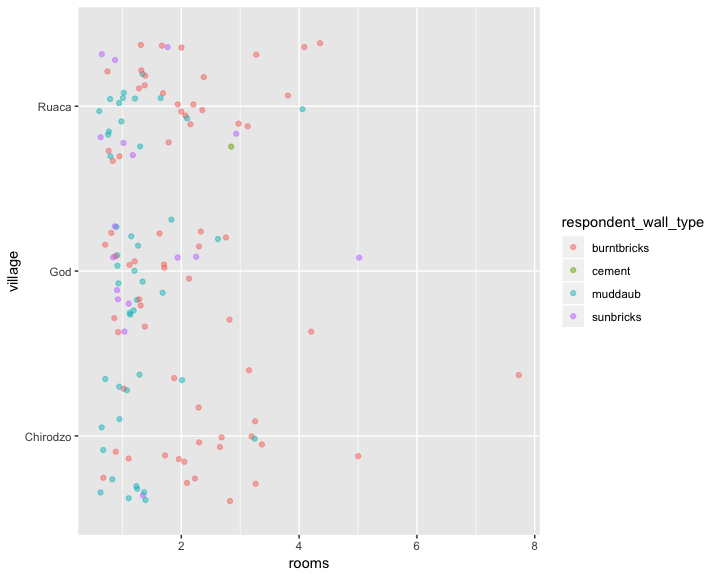
\includegraphics[width=10cm]{Screenshot36.png}
    \label{fig:ls-36}
\end{figure}

No, it is not a good way to plot data

Objective: Replace the box plot with a violin plot; see geom_violin().
Solution

Action:

\begin{verbatim}ggplot(data = interviews_plotting, aes(x = respondent_wall_type, y = rooms)) +
    geom_violin(alpha = 0) +
    geom_jitter(alpha = 0.5, color = "tomato")
\end{verbatim}
Result:

\begin{figure}[htp]
    \centering
    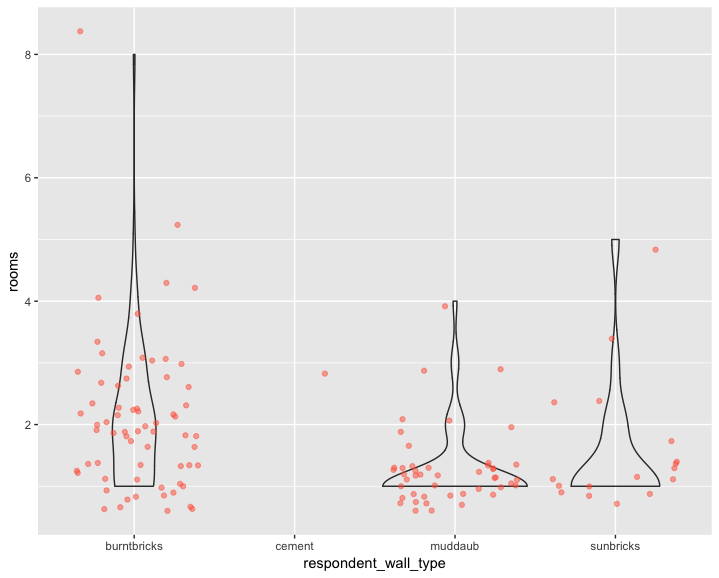
\includegraphics[width=10cm]{Screenshot37.png}
    \label{fig:ls-37}
\end{figure}

Objective: Create a boxplot for liv_count for each wall type. Overlay the boxplot layer on a jitter layer to show actual measurements.

Action:

\begin{verbatim}ggplot(data = interviews_plotting, aes(x = respondent_wall_type, y = liv_count)) +
    geom_boxplot(alpha = 0) +
    geom_jitter(alpha = 0.5)
\end{verbatim}
Result:

\begin{figure}[htp]
    \centering
    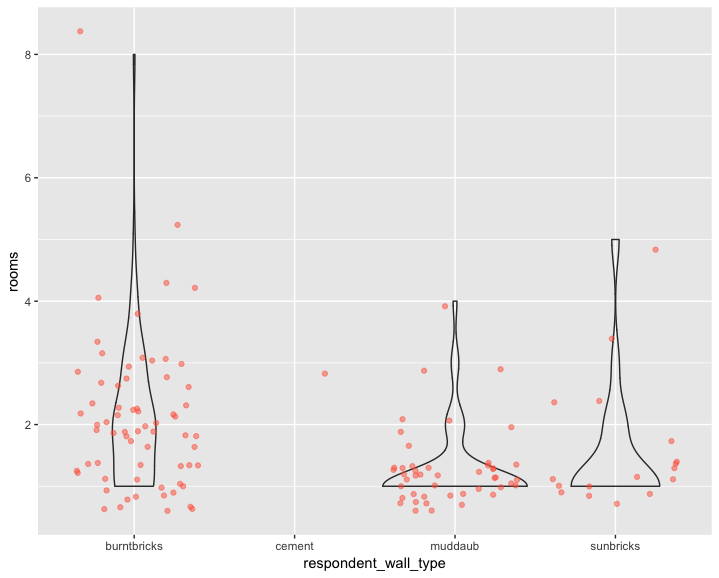
\includegraphics[width=10cm]{Screenshot37.png}
    \label{fig:ls-38}
\end{figure}

Objective: Add color to the data points on your boxplot according to whether the respondent is a member of an irrigation association.

Action:

\begin{verbatim}ggplot(data = interviews_plotting, aes(x = respondent_wall_type, y = liv_count)) +
    geom_boxplot(alpha = 0) +
    geom_jitter(alpha = 0.5, color = "memb_assoc")
\end{verbatim}
Error: Error in grDevices::col2rgb(colour, TRUE) : 
  invalid color name 'memb_assoc' \label{sec: colourdatapoints}

Action:

\begin{verbatim}ggplot(data = interviews_plotting, aes(x = respondent_wall_type, y = liv_count)) +
    geom_boxplot(alpha = 0) +
    geom_jitter(aes(alpha = 0.5, color = memb_assoc))
\end{verbatim}
Result:

\begin{figure}[htp]
    \centering
    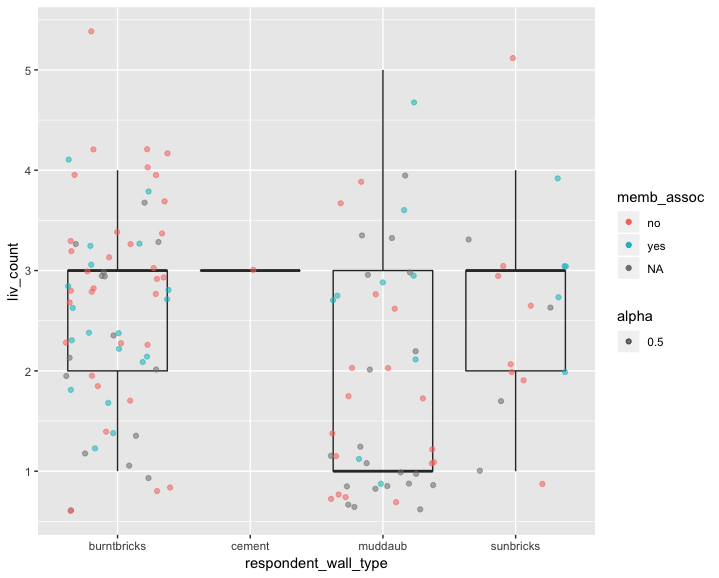
\includegraphics[width=10cm]{Screenshot39.png}
    \label{fig:ls-39}
\end{figure}

Objective: Create a bar plot showing the proportion of respondents in each village who are or are not part of an irrigation association (memb_assoc). Include only respondents who answered that question in the calculations and plot. Which village had the lowest proportion of respondents in an irrigation association?

Action:

\begin{verbatim}percent_memb_assoc <- interviews_plotting %>%
 filter(!is.na(memb_assoc)) %>%
  count(village, memb_assoc) %>%
  group_by(village) %>%
  mutate(percent = n / sum(n)) %>%
  ungroup()

ggplot(percent_memb_assoc, aes(x = village, y = percent, fill = memb_assoc)) +
geom_bar(stat = "identity", position = "dodge")
\end{verbatim}
Result:

\begin{figure}[htp]
    \centering
    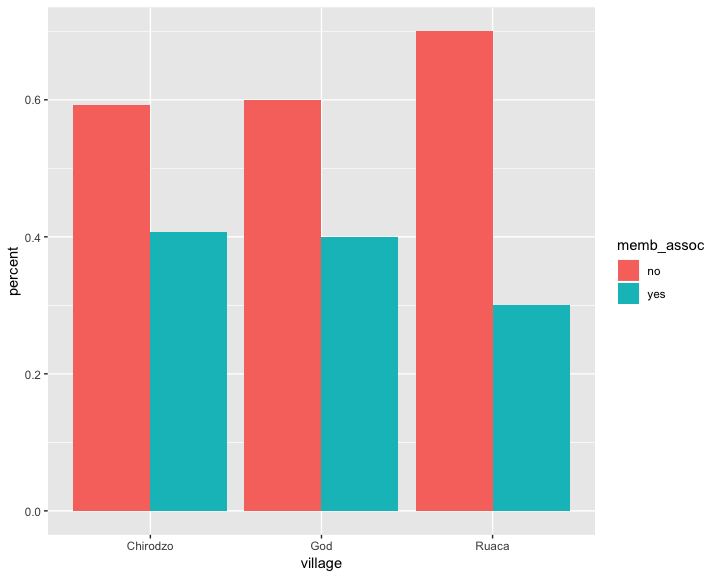
\includegraphics[width=10cm]{Screenshot40.png}
    \label{fig:ls-40}
\end{figure}

Ruaca had the lowest proportion of respondents who weren't in an irrigation association.

Objective: Experiment with two themes from https://ggplot2.tidyverse.org/reference/ggtheme.html

Action:

\begin{verbatim}percent_items <- interviews_plotting %>%
    gather(items, items_owned_logical, bicycle:no_listed_items) %>%
    filter(items_owned_logical) %>%
    count(items, village) %>%
    ## add a column with the number of people in each village
    mutate(people_in_village = case_when(village == "Chirodzo" ~ 39,
                                         village == "God" ~ 43,
                                         village == "Ruaca" ~ 49)) %>%
    mutate(percent = n / people_in_village)

mutate(percent = n / people_in_village)
ggplot(percent_items, aes(x = village, y = percent)) +
  geom_bar(stat = "identity", position = "dodge") +
  facet_wrap(~ items) +
  theme_dark() +
  theme(panel.grid = element_blank())

mutate(percent = n / people_in_village)
ggplot(percent_items, aes(x = village, y = percent)) +
  geom_bar(stat = "identity", position = "dodge") +
  facet_wrap(~ items) +
  theme_light() +
  theme(panel.grid = element_blank())
\end{verbatim}
Result:

\begin{figure}[htp]
    \centering
    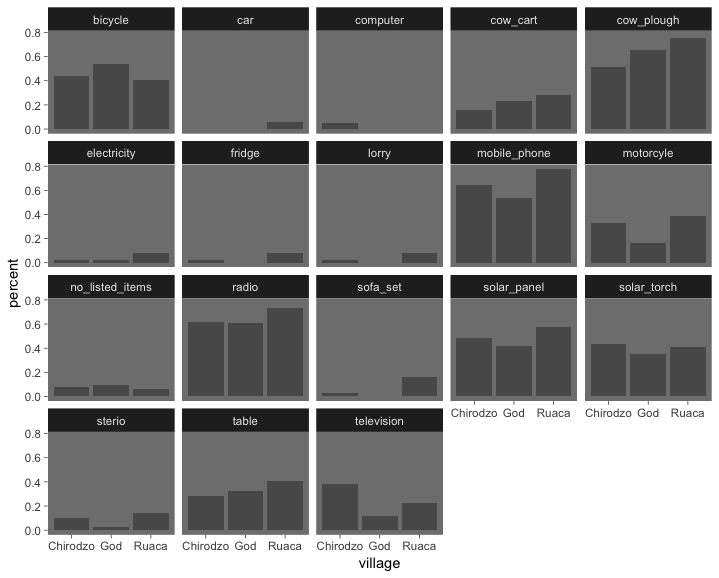
\includegraphics[width=10cm]{Screenshot41.png}
    \label{fig:ls-41}
\end{figure}

\begin{figure}[htp]
    \centering
    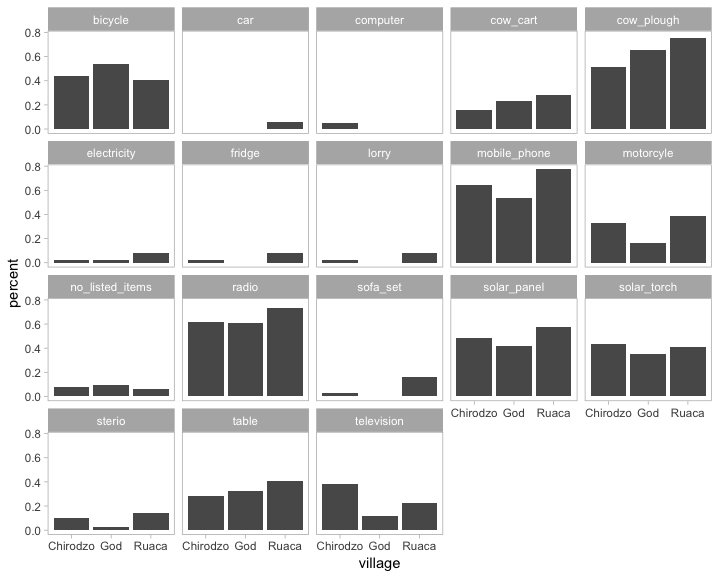
\includegraphics[width=10cm]{Screenshot42.png}
    \label{fig:ls-42}
\end{figure}

I prefer theme light. 

Objective: Create own plot

Action:

\begin{verbatim}
my_plot <- ggplot(percent_items, aes(x = village, y = percent, fill = village)) +
  geom_bar(stat = "identity", position = "dodge") +
  facet_wrap(~ items) +
  labs(title = "Percent of respondents in each village \n who owned each item",
       x = "Village",
       y = "Percent of Respondents") +
  theme(axis.text.x = element_text(size = 12, angle = 45, hjust = 0.5, vjust = 0.5),
        axis.text.y = element_text(size = 12),
        text = element_text(size = 12),
        plot.title = element_text(hjust = 0.2))

ggsave("fig_output/name_of_file.png", my_plot, width = 15, height = 10)
\end{verbatim}
Result:

\begin{figure}[htp]
    \centering
    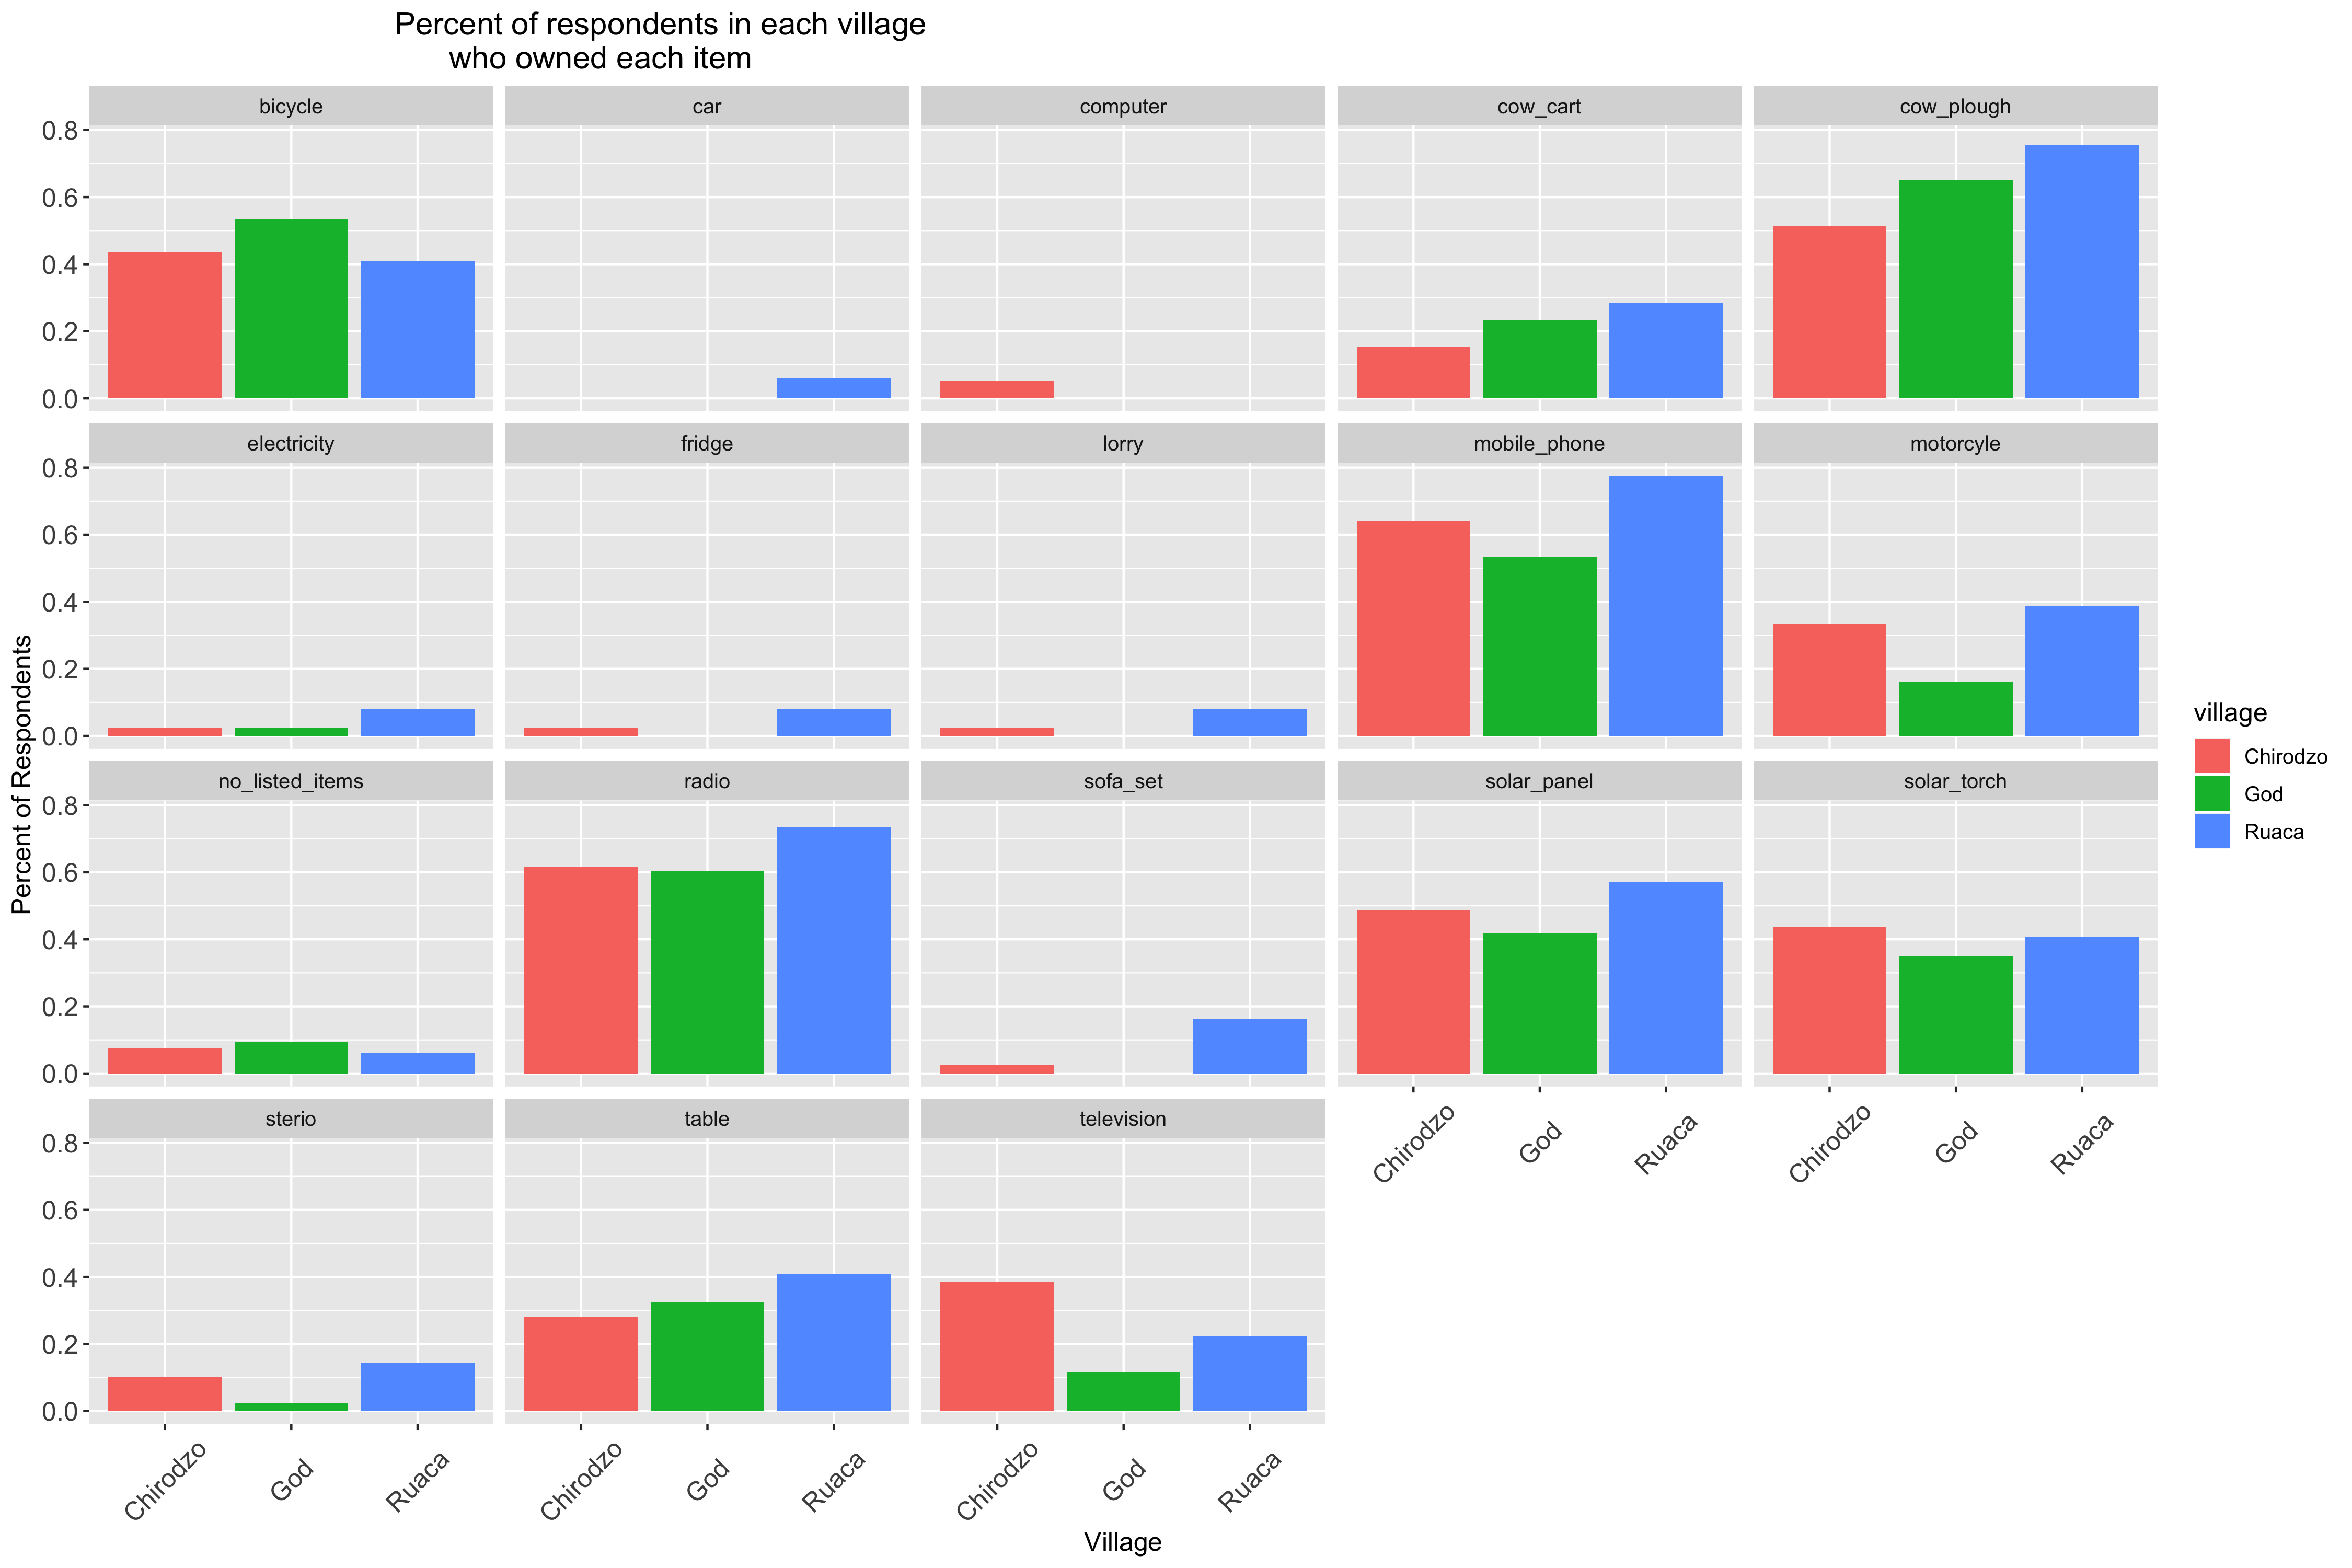
\includegraphics[width=10cm]{Screenshot43.png}
    \label{fig:ls-43}
\end{figure}


\begin{verbatim}
\end{verbatim}

\newpage
\section{Class notes and other homework}
\subsection*{12/8/2019 - 8:45pm}
\subsubsection*{Homework Exercise}
We were asked to think of two examples of problem data produced by our discipline. For sociology, the two that come to mind is data from surveys and secondary data sources such as government statistics. I may use neither for my own thesis research proposal so have outlined theoretical issues based on what I know.\par
While surveys can yield significant data, it depends on the exact questions asked and the available answers. Surveys may not capture how people act but rather what they think or believe they should think.\par
Quantitative surveys may not have an option that reflects the interviewees actual response. Qualitative surveys provide more options but bad coding of answers by the interviewer may twist responses into something that do not reflect what was said.\par
Data using secondary sources is often used but there can be problems. Using different datasets that might have different assumptions, for example, trying to use old government statistical data over a long time period when the collection method and calculations have changed.

\subsection*{16/8/2019 - 2:10pm}
\subsubsection*{FOAR705 Week 3 Class}
Revised date for scoping study. Scoping study uploaded to Cloudstor can be deleted. Contact Brian on DM to get it deleted from iLearn on Slack.\par
If you don’t define the problem, you won’t know if you have solved it.\par
Scoping is what is the point of the exercise. The aim is to think about the problem without the context of the solution.\par
Stackoverflow aimed at being a site to ask about problem, not solutions.\par
Elaboration is about identifying what technology (tool or technique) has solved the problem e.g. checklist is a technology. The aim is to not invent things from scratch and find how most people have solved a similar problem.\par
Test technology to see if we understood its claims correctly as it can be portrayed with rose coloured glasses.\par
Note that 80-90\% of software products fail.\par
Thesis is a project. If you don’t define the problem the thesis will face, you won’t know.\par
Formatting cannot have meaning.\par
Controlled vocabulary - saying at the start, the only options that can be chosen. Any other value is an error. There is a prepopulated list (allows Other).\par
Each variable should have an explanation in metadata.\par
Metadata is a description of your dataset such that someone will be able to add to it. Sufficiently detailed that someone can add a new row.\par
Metadata is not just for spreadsheets e.g. bibliography - where did we look, what search terms did use to we find it. Readme file - file name and description in folder.\par
Metadata should be in a different file, not a table. If you save something as a CSV, formatting is gone and you cannot have tabs.\par

\subsection*{16/8/2019 - 3:16pm}
\subsubsection*{FOAR705 Week 3 Class - Computational Thinking}

Computation thinking:\par
Decomposition - Taking a complex task and breaking it down into what needs to be done\par
Algorithm Design: articulating set of step-by-step instructions\par
Properly formatted references and bibliography exercise. Tasks to be done?
\begin{itemize}
\item Define what properly formatted and bibliography mean in terms of my thesis
\item Find required format
\item Getting the correct information in
\end{itemize}
Humans are good at collecting data, summarisation is tedious.
\subsection*{16/8/2019 - 3:16pm} 
\subsubsection*{FOAR705 Week 3 Class - Project Management Notes}
\begin{itemize}
\item Waterfall vs agile approach
\item Agile manifesto - not fetishing the process
\item Before investing time, fail early and often and test. Develop a couple of steps and test them. If they do not work, you may have to start over.
\item Do preliminary work to see if it is going to work. Respond to changes and feedback.
\item Estimate how much time each sub-task takes on Gantt chart so you can make adjustments. It is about identifying what is the critical path.
\item Kanban board can break down sub-tasks into what you need to do daily and can complement Gantt charts.
\item Kanban can limit your work in progress.
\end{itemize}

\subsection*{24/8/2019 - 5:34pm} 
\subsubsection*{Adding Images to LaTex} 

The use of Bash means I need to screenshot results rather than try to type it out.

Overleaf provided some instructions and code for it at \begin{verbatim}https://www.overleaf.com/learn/how-to/Including_images_on_Overleaf\end{verbatim} 

Firstly the screenshot needs to be uploaded before the following code is entered: 

\begin{verbatim}\begin{figure}[htp]
    \centering
    \includegraphics[width=xcm]{imagename.png}
    \label{fig:imagename}
\end{figure}
\end{verbatim}

\subsection*{6/8/2019 - 3:06pm} 
\subsubsection*{Proof of Concept - Design} 

Individual components working by Week 9 to then work together by Week 11.

Design document

Elaboration is not a to-do list, it was a superficial look at tools

Take decomposition and apply it to proof of concept.

Breaking down tasks that need to be achieved to as part of a set of user stories.

Acceptance criteria are is a recipe that someone else can follow.

Stories can categorise them

Load into a project management system. Can do Github or Trello

Then share user stories for feedback from colleagues. Does it make sense? To tease out ambiguities.

More than 10 user stories, less than 30 stories.

Description not in the user story but have elsewhere

No ambiguity, no advanced thought.


That I have a second Duplicati backup that points at an external hard drive and a calendar reminder to do that.

Where to put the user stories


TRELLO:

Title is user story

Description is acceptance criteria

Comments are actions I have taken as a log

Lack of priority - which things to do in which order. Can use Trello via labels to do this.

User Stories include setup so do it for

Before index need to set up - treat as a user story


VM setup - instructions e.g. you should do X for API.




Automated testing

Unit Test - reading

Attempts 

Simplest thing - have something like a screen rec

Play with Automator for quality assurance test.



User Acceptance Test.

All these stories into a to do-list

Automation get a computer to do it


Licence file and readme

Put a licence in a respository of your code and 

Readme in repository.

Quick pitch about what you done.

User story - separate for export


Git-Repository

Shellscript that uses

Shared Folder as documents as a test

Instructions for users

Techniques for the human to achieve the goal.

Shellscript to download everything in a mac

Tag hierarchies

Save automation testing scripts

Figure out how to export file and how to write a code to import it into a Zotero

Export of hypothes.is 

Download uploaded to program in Zotero via R?

Upload vocabulry

Tag list





Document

Tag naming framework document

Virtual




\end{document}
